\chapter{内点法}
\label{chap:lp-interior-point}

第~\ref{chap:simplex-method}章的工厂问题里，单纯形法从原点出发，沿可行域的边走过几个顶点，到达最优顶点$(4,2)$。每到一个顶点，都要决定下一步走哪条边。顶点的数目可以随维数指数增长，第~\ref{chap:simplex-method}章末尾的构造说明，这种逐个顶点的走法在最坏情形下确实可能走遍它们。于是有一个自然的问题：能不能不贴着边走，而从可行域的中间穿过去？

穿过中间要解决三件事。一是在内部靠什么指路：内部的每个点都可行，目标又是线性的，梯度处处相同，单看目标看不出该往哪里停。二是怎样防止撞上边界，同时又让终点能落在边界上，因为线性规划的最优解总在边界上。三是走到什么程度算完：内部的点永远不会恰好是顶点，“差不多最优”要有能核对的含义。

本章的回答是第~\ref{chap:linear-programming}章对偶理论的一个直接延伸。把互补松弛条件$x_is_i=0$放宽成$x_is_i=\mu$，再让正数$\mu$逐渐减小到零，方程组的解就连成一条从内部通向最优面的光滑曲线。第一节建立这条曲线，第二节用Newton法沿它前进，并在一个能手算的小例子上逐轮写出全部计算。

后面四节处理算法落地时的问题。起点从哪里来，放在第三节；三项残差怎样决定停止、近似解怎样变成基和严格证书，放在第四节；第五节证明一种路径跟踪规则的迭代次数只随$\sqrt{n}$增长，并说明这和线性规划的多项式可解性是什么关系；最后一节在工厂问题上把内点法和单纯形法放在一起比较。一般非线性约束上的内点法由第~\ref{chap:nonlinear-interior-point}章讨论。

\section{中心路径}
\label{sec:lpipm-central-path}

在可行域内部，沿怎样一条路线走，才能既不撞上边界，又最终到达最优解？答案是一条由对偶理论确定的曲线。我们先回顾要用到的对偶事实，再从一维的障碍函数讲起。

\paragraph{标准型与对偶}
本章讨论第~\ref{chap:linear-programming}章的标准型线性规划及其对偶：
\begin{equation}
 \min_{\bm{x}}\ \bm{c}^\top\bm{x}\quad\text{s.t.}\quad\bm{A}\bm{x}=\bm{b},\quad\bm{x}\geq\bm{0},
 \label{eq:lpipm-primal}
\end{equation}
\begin{equation}
 \max_{\bm{y},\bm{s}}\ \bm{b}^\top\bm{y}\quad\text{s.t.}\quad\bm{A}^\top\bm{y}+\bm{s}=\bm{c},\quad\bm{s}\geq\bm{0},
 \label{eq:lpipm-dual}
\end{equation}
其中$\bm{A}\in\mathbb{R}^{m\times n}$满行秩，$\bm{y}\in\mathbb{R}^m$无符号限制，$\bm{s}\in\mathbb{R}^n$称为对偶松弛。两个最优值分别记为$p^\star$和$d^\star$。

那一章的两个结论是本章的出发点。第一个是目标差的恒等式：若$\bm{x}$原始可行，$(\bm{y},\bm{s})$对偶可行，把$\bm{c}=\bm{A}^\top\bm{y}+\bm{s}$和$\bm{b}=\bm{A}\bm{x}$代入目标差，得到
\begin{equation}
 \bm{c}^\top\bm{x}-\bm{b}^\top\bm{y}
 =(\bm{A}^\top\bm{y}+\bm{s})^\top\bm{x}-(\bm{A}\bm{x})^\top\bm{y}
 =\bm{x}^\top\bm{s}.
 \label{eq:lpipm-gap-identity}
\end{equation}
左边称为对偶间隙。因为$\bm{x},\bm{s}\geq\bm{0}$，它非负，这就是弱对偶。

第二个是强对偶：问题可行且最优值有限时，$p^\star=d^\star$。于是$(\bm{x},\bm{y},\bm{s})$最优，当且仅当它同时满足
\begin{equation}
 \bm{A}\bm{x}=\bm{b},\qquad\bm{A}^\top\bm{y}+\bm{s}=\bm{c},\qquad x_is_i=0\ (i=1,\ldots,n),\qquad\bm{x},\bm{s}\geq\bm{0}.
 \label{eq:lpipm-kkt}
\end{equation}
中间的条件是互补松弛。前两组方程是线性的，难处全在$x_is_i=0$：对每个下标，要决定是$x_i$为零还是$s_i$为零。这是一个组合选择，单纯形法用基来做这个选择，一次换基改动一个下标。

全章贯穿下面这个小例子，只有一条等式约束：
\begin{equation}
 \min_{\bm{x}}\ x_1+2x_2+3x_3\quad\text{s.t.}\quad x_1+x_2+x_3=1,\quad\bm{x}\geq\bm{0}.
 \label{eq:lpipm-running}
\end{equation}
这里$n=3$，$m=1$，$\bm{A}=[1\ 1\ 1]$，$b=1$，$\bm{c}=(1,2,3)^\top$。可行集是$\mathbb{R}^3$中以三个单位向量为顶点的三角形。

对偶约束是$y+s_i=c_i$，即$\bm{s}=(1-y,\,2-y,\,3-y)^\top$，$\bm{s}\geq\bm{0}$等价于$y\leq1$，对偶目标就是$y$本身。最优解和最优对偶解都一眼可得：
\[
 \bm{x}^\star=(1,0,0)^\top,\qquad y^\star=1,\qquad\bm{s}^\star=(0,1,2)^\top,\qquad p^\star=d^\star=1.
\]
可以核对$x_i^\star s_i^\star$全为零。

\paragraph{贴边走与穿过去}
图~\ref{fig:lpipm-edge-vs-interior}是第~\ref{chap:simplex-method}章的工厂问题。黄线是单纯形法的路线，它贴着边界，在三个拐角上各做了一次选择。绿线是本节要建立的路径，它从内部一个点出发，平滑地弯向最优顶点，途中不需要决定任何“走哪条边”的问题。

可以把可行域想成一间房间，最优解在墙角。贴墙走，每到拐角都要判断往哪边转；从房间中央穿过去，没有拐角，但需要两样东西：一种不让人撞墙的力，以及一种随时间减弱这个力的办法，否则永远到不了墙角。这个比喻在终点处失效：真正的解就在墙上，所以排斥力必须在极限中消失，下面的$\mu\downarrow0$就是这件事。

\begin{BookInlineFigure}
  \centering
  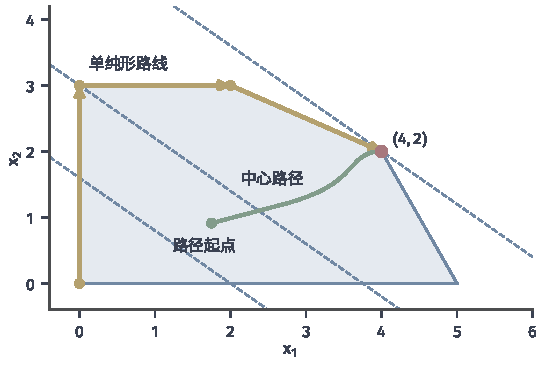
\includegraphics[width=92mm]{figures/05-optimization/01-linear-programming/matplotlib/lpipm-edge-vs-interior/figure.pdf}
  \caption{工厂问题的两条路线。浅蓝区域是可行域，蓝色虚线是利润的等值线，红点是最优顶点$(4,2)$。黄线是单纯形法经过的顶点序列$(0,0)$、$(0,3)$、$(2,3)$、$(4,2)$；绿线是中心路径，从$\mu$很大时的内部点出发，随$\mu$减小弯向最优顶点，全程不碰边界。}
  \label{fig:lpipm-edge-vs-interior}
\end{BookInlineFigure}

\paragraph{一维的障碍}
先看最简单的情形：在$x\geq0$上最小化$f(x)=x$，解是边界点$x=0$。在目标上加一项$-\mu\log x$，其中$\mu>0$，它在$x\downarrow0$时趋于$+\infty$，像一堵逐渐升高的墙，把迭代挡在$x>0$的一侧。这时要解的是
\[
 \min_{x>0}\ x-\mu\log x.
\]
令导数$1-\mu/x$为零，得到唯一的最小点
\[
 x=\mu.
\]
图~\ref{fig:lpipm-log-barrier}显示了两件事。图(a)中，$\mu$越小，墙贴得越紧，离墙稍远的地方几乎不受影响。图(b)中，绿点是加了障碍后的最小点，它随$\mu$减小沿$x=\mu$滑向真正的解$x=0$。

\begin{BookInlineFigure}
  \centering
  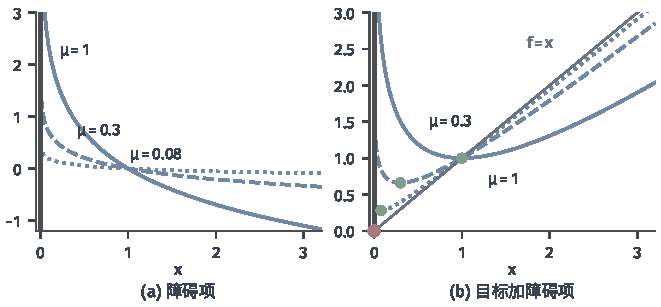
\includegraphics[width=112mm]{figures/05-optimization/01-linear-programming/matplotlib/lpipm-log-barrier/figure.pdf}
  \caption{一维的对数障碍。(a)障碍项$-\mu\log x$，实线、虚线、点线分别对应$\mu=1,0.3,0.08$，深灰粗线是边界$x=0$。(b)目标$f(x)=x$（细灰线）加上障碍项后的三条曲线，绿点是各自的最小点$x=\mu$，红点是真正的解$x=0$。}
  \label{fig:lpipm-log-barrier}
\end{BookInlineFigure}

\paragraph{对数障碍问题}
回到问题~\eqref{eq:lpipm-primal}，对每个坐标都加一项障碍。这里要留意“内部”的含义。例~\eqref{eq:lpipm-running}的可行集是$\mathbb{R}^3$中的一块三角形，厚度为零，没有通常意义下的内点。障碍只负责不等式$\bm{x}\geq\bm{0}$，等式$\bm{A}\bm{x}=\bm{b}$始终严格保持，所以内部是相对等式约束而言的，指满足等式且所有分量为正的点。

\begin{definition}[严格可行]
\label{def:lpipm-strictly-feasible}
满足$\bm{A}\bm{x}=\bm{b}$且$\bm{x}>\bm{0}$的点称为原始\term{严格可行}（strictly feasible）点。满足$\bm{A}^\top\bm{y}+\bm{s}=\bm{c}$且$\bm{s}>\bm{0}$的$(\bm{y},\bm{s})$称为对偶严格可行点。两者都存在时，记
\begin{equation}
 \mathcal{F}^{\circ}=\bigl\{(\bm{x},\bm{y},\bm{s}):\bm{A}\bm{x}=\bm{b},\ \bm{A}^\top\bm{y}+\bm{s}=\bm{c},\ \bm{x}>\bm{0},\ \bm{s}>\bm{0}\bigr\}.
 \label{eq:lpipm-strict-set}
\end{equation}
\end{definition}

严格可行点不一定存在。约束$x_1+x_2=0$、$\bm{x}\geq\bm{0}$的可行集只有原点，其中没有正的点。例~\eqref{eq:lpipm-running}中，$\bm{x}=(1/3,1/3,1/3)^\top$与$y=0$、$\bm{s}=(1,2,3)^\top$都严格可行。

对$\mu>0$，定义\term{对数障碍}（logarithmic barrier）问题
\begin{equation}
 \min_{\bm{x}}\ B_\mu(\bm{x})=\bm{c}^\top\bm{x}-\mu\sum_{i=1}^n\log x_i
 \quad\text{s.t.}\quad\bm{A}\bm{x}=\bm{b},\quad\bm{x}>\bm{0}.
 \label{eq:lpipm-barrier}
\end{equation}
图~\ref{fig:lpipm-bowls}画出例~\eqref{eq:lpipm-running}中$B_\mu$的等值线。线性目标本身没有碗底，障碍项在三条边上竖起墙，围出一个碗。$\mu$大时碗底靠近三角形中央，$\mu$小时墙贴向边界，碗底被线性目标推向最优顶点。

\begin{BookInlineFigure}
  \centering
  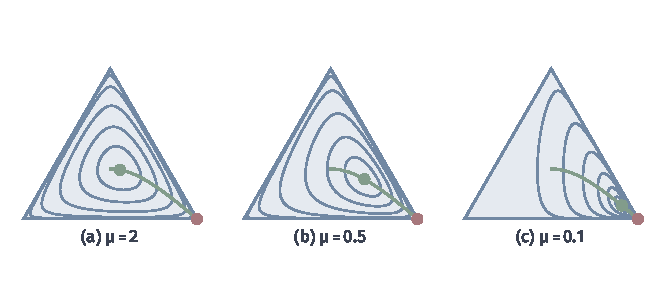
\includegraphics[width=112mm]{figures/05-optimization/01-linear-programming/matplotlib/lpipm-bowls/figure.pdf}
  \caption{例~\eqref{eq:lpipm-running}的障碍目标$B_\mu$在三角形上的等值线（蓝线）。绿线是全部碗底连成的曲线，绿点是当前$\mu$的碗底，红点是最优顶点。$\mu$减小时，碗底沿绿线向红点移动，碗也越来越贴近边界。}
  \label{fig:lpipm-bowls}
\end{BookInlineFigure}

\paragraph{一阶条件给出扰动的互补}
$B_\mu$的梯度是$\bm{c}-\mu\bm{X}^{-1}\bm{1}$，其中$\bm{X}=\operatorname{diag}(\bm{x})$，$\bm{1}$是全一向量。在仿射集合$\{\bm{x}:\bm{A}\bm{x}=\bm{b}\}$上，能移动的方向是$\bm{A}$的零空间，一阶条件要求梯度与零空间正交。$\bm{A}$的零空间的正交补是$\bm{A}^\top$的列空间，所以一阶条件是：存在$\bm{y}$使
\[
 \bm{c}-\mu\bm{X}^{-1}\bm{1}=\bm{A}^\top\bm{y}.
\]

这里出现了一个与$\bm{c}-\bm{A}^\top\bm{y}$相等的正向量，正是对偶松弛的样子。令$\bm{s}=\mu\bm{X}^{-1}\bm{1}$，上式成为$\bm{A}^\top\bm{y}+\bm{s}=\bm{c}$，而$\bm{s}$的定义就是$x_is_i=\mu$。三组条件合起来是
\begin{equation}
 \bm{A}\bm{x}=\bm{b},\qquad\bm{A}^\top\bm{y}+\bm{s}=\bm{c},\qquad x_is_i=\mu\ (i=1,\ldots,n),\qquad\bm{x},\bm{s}>\bm{0}.
 \label{eq:lpipm-central}
\end{equation}
把它与最优性条件~\eqref{eq:lpipm-kkt}逐项对比，只有互补松弛一处不同：$x_is_i=0$换成了$x_is_i=\mu$。

图~\ref{fig:lpipm-complementarity-corner}说明这个改动的好处。在$(x_i,s_i)$平面上，$x_is_i=0$、$x_i,s_i\geq0$是一个直角折线，组合选择就是选落在哪条腿上。把它换成双曲线$x_is_i=\mu$，折角被磨圆了，曲线是光滑的，可以用微积分处理；$\mu$越小，曲线越贴近折角。

\begin{BookInlineFigure}
  \centering
  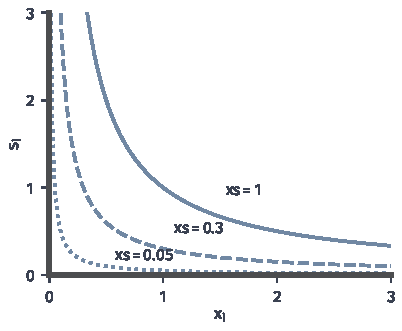
\includegraphics[width=68mm]{figures/05-optimization/01-linear-programming/matplotlib/lpipm-complementarity-corner/figure.pdf}
  \caption{互补条件的光滑化。深灰粗线是$x_is_i=0$、$x_i,s_i\geq0$的直角折线，蓝色曲线是$x_is_i=\mu$，实线、虚线、点线分别对应$\mu=1,0.3,0.05$。$\mu\downarrow0$时曲线贴近折线，但对每个正的$\mu$，$x_i$和$s_i$都严格为正。}
  \label{fig:lpipm-complementarity-corner}
\end{BookInlineFigure}

\paragraph{存在唯一的条件}
碗底并不总是存在，下面的定理说明它需要原始和对偶两侧都有严格可行点。

\begin{theorem}[中心点的存在唯一]
\label{thm:lpipm-central-exists}
设$\bm{A}$满行秩，$\mu>0$。方程组~\eqref{eq:lpipm-central}有解，当且仅当$\mathcal{F}^{\circ}$非空。此时解$(\bm{x}(\mu),\bm{y}(\mu),\bm{s}(\mu))$唯一，且$\bm{x}(\mu)$是障碍问题~\eqref{eq:lpipm-barrier}的唯一最小点。
\end{theorem}

\begin{proof}
必要性：方程组的解本身就是$\mathcal{F}^{\circ}$中的点。

充分性分两步。先证最小点存在。取$(\bar{\bm{y}},\bar{\bm{s}})$对偶严格可行，在原始可行点上，由$\bm{c}=\bm{A}^\top\bar{\bm{y}}+\bar{\bm{s}}$和$\bm{A}\bm{x}=\bm{b}$，目标可以改写为
\[
 \bm{c}^\top\bm{x}=\bm{b}^\top\bar{\bm{y}}+\bar{\bm{s}}^\top\bm{x},
\]
于是
\[
 B_\mu(\bm{x})=\bm{b}^\top\bar{\bm{y}}+\sum_{i=1}^n\bigl(\bar{s}_ix_i-\mu\log x_i\bigr).
\]
因为$\bar{s}_i>0$，每个一元函数$\bar{s}_it-\mu\log t$在$(0,\infty)$上有下界，并且在$t\downarrow0$和$t\to\infty$时都趋于$+\infty$。

于是对原始严格可行点$\bm{x}^{(0)}$，考虑下水平集
\[
 \bigl\{\bm{x}:\bm{A}\bm{x}=\bm{b},\ \bm{x}>\bm{0},\ B_\mu(\bm{x})\leq B_\mu(\bm{x}^{(0)})\bigr\}.
\]
其中每个坐标都落在某个区间$[\epsilon,R]$内，$\epsilon>0$，这是非空紧集。连续函数在紧集上取到最小值，这就是障碍问题的一个最小点。

再证一阶条件与最小点等价，并得到唯一性。最小点在相对内部，一阶条件成立，于是得到方程组~\eqref{eq:lpipm-central}的一个解。反过来，设$(\bm{x},\bm{y},\bm{s})$是一个解。函数$-\log t$是凸函数，所以$B_\mu$在可行集上是严格凸的，对任何可行的$\bm{x}'$有
\[
 B_\mu(\bm{x}')\geq B_\mu(\bm{x})+\nabla B_\mu(\bm{x})^\top(\bm{x}'-\bm{x})=B_\mu(\bm{x})+\bm{y}^\top\bm{A}(\bm{x}'-\bm{x})=B_\mu(\bm{x}),
\]
这说明$\bm{x}$是最小点。严格凸性保证最小点唯一，于是$\bm{x}$唯一，$\bm{s}=\mu\bm{X}^{-1}\bm{1}$也唯一。$\bm{A}^\top$列满秩，$\bm{A}^\top\bm{y}=\bm{c}-\bm{s}$给出唯一的$\bm{y}$。
\end{proof}

对偶严格可行这个条件不能省。问题$\min 0$、$x_1-x_2=0$、$\bm{x}\geq\bm{0}$有原始严格可行点$(1,1)$，最优值为$0$。它的障碍目标在可行射线$x_1=x_2=r$上等于$-2\mu\log r$，当$r\to\infty$时趋于$-\infty$，没有最小点。原因在对偶一侧：对偶约束$y+s_1=0$、$-y+s_2=0$迫使$s_1+s_2=0$，严格可行点不存在。

\begin{definition}[中心路径]
\label{def:lpipm-central-path}
当$\mathcal{F}^{\circ}$非空时，$\mu$取遍$(0,\infty)$，方程组~\eqref{eq:lpipm-central}的解构成一条曲线
\begin{equation}
 \mathcal{C}=\bigl\{(\bm{x}(\mu),\bm{y}(\mu),\bm{s}(\mu)):\mu>0\bigr\},
 \label{eq:lpipm-central-path}
\end{equation}
称为\term{中心路径}（central path）。其中的点称为中心点。
\end{definition}

这个名字可以这样理解：方程组要求所有乘积$x_is_i$相等，没有哪个坐标比别的坐标更靠近自己的边界，点保持在“中央”。下面的例子把路径完整地写出来。

\begin{example}[贯穿例的中心路径]
\label{ex:lpipm-central-closed-form}
在问题~\eqref{eq:lpipm-running}中，$s_i=c_i-y$，$x_is_i=\mu$给出$x_i=\mu/(c_i-y)$。代入$x_1+x_2+x_3=1$，消去$\bm{x}$，得到$\mu$与$y$的关系
\[
 \mu=\Bigl(\frac{1}{1-y}+\frac{1}{2-y}+\frac{1}{3-y}\Bigr)^{-1},\qquad y<1.
\]
所以路径可以用$y$作参数直接写出。

取$y=0$，则$\bm{s}=(1,2,3)^\top$，括号内是$1+\tfrac12+\tfrac13=\tfrac{11}{6}$，于是
\[
 \mu=\frac{6}{11},\qquad\bm{x}=\Bigl(\frac{6}{11},\frac{3}{11},\frac{2}{11}\Bigr)^\top.
\]
三个乘积都等于$6/11$，三个分量之和为$1$。

再取$y=1/2$，则$\bm{s}=(\tfrac12,\tfrac32,\tfrac52)^\top$，括号内是$2+\tfrac23+\tfrac25=\tfrac{46}{15}$，于是
\[
 \mu=\frac{15}{46},\qquad\bm{x}=\Bigl(\frac{15}{23},\frac{5}{23},\frac{3}{23}\Bigr)^\top.
\]

两端的行为也能读出来。$y\to-\infty$时$\mu\to\infty$，$x_i$趋于相等，极限是$(1/3,1/3,1/3)^\top$。$y\uparrow1$时第一项发散，$\mu\to0$，$\bm{x}\to(1,0,0)^\top$。
\end{example}

图~\ref{fig:lpipm-central-path}把这条路径画在三角形上。起点是$\mu\to\infty$的极限，这一点最大化$\sum_i\log x_i$，称为可行集的\term{解析中心}（analytic center）。解析中心只有在可行集有界时才存在，它只由约束决定，与目标无关；目标$\bm{c}$的作用是决定路径离开中心后朝哪里弯。

\begin{BookInlineFigure}
  \centering
  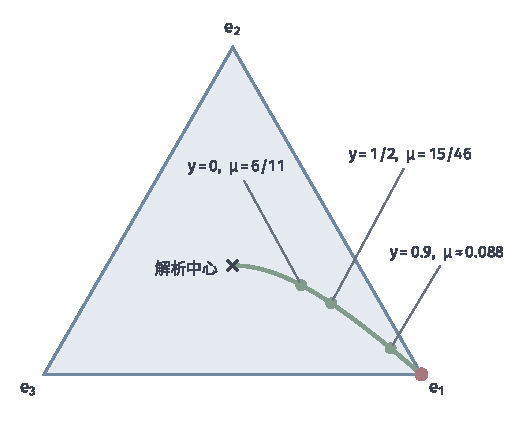
\includegraphics[width=90mm]{figures/05-optimization/01-linear-programming/matplotlib/lpipm-central-path/figure.pdf}
  \caption{贯穿例的中心路径。三角形是可行集，三个角是单位向量，黑叉是解析中心$(1/3,1/3,1/3)^\top$，绿线是中心路径，绿点是例~\ref{ex:lpipm-central-closed-form}算出的中心点以及$y=0.9$的中心点，红点是最优顶点$\bm{e}_1$。}
  \label{fig:lpipm-central-path}
\end{BookInlineFigure}

\paragraph{间隙恰好是$n\mu$}
中心路径最有用的性质是，沿路径的对偶间隙可以直接读出来。中心点原始、对偶都可行，把式~\eqref{eq:lpipm-gap-identity}用到这里，再代入$x_is_i=\mu$，得到
\begin{equation}
 \bm{c}^\top\bm{x}(\mu)-\bm{b}^\top\bm{y}(\mu)=\sum_{i=1}^nx_i(\mu)s_i(\mu)=n\mu.
 \label{eq:lpipm-central-gap}
\end{equation}

它把“还差多远”变成了一个已知的数。由弱对偶$\bm{b}^\top\bm{y}(\mu)\leq p^\star$，原始目标误差不超过间隙：
\begin{equation}
 \bm{c}^\top\bm{x}(\mu)-p^\star\leq n\mu.
 \label{eq:lpipm-central-error}
\end{equation}
要让误差不超过$\varepsilon$，走到$\mu\leq\varepsilon/n$就够了。在例~\ref{ex:lpipm-central-closed-form}中，$y=0$的中心点目标值是$6/11+6/11+6/11=18/11$，对偶目标是$0$，间隙$18/11$正好等于$3\mu$。

这个结论用到了精确的中心点。迭代算法只能走到中心路径附近，这时间隙怎样计算，第~\ref{sec:lpipm-accuracy}节会逐项说明。

\paragraph{路径的终点}
式~\eqref{eq:lpipm-central-gap}说明目标值收敛到最优值，却没有说点本身收敛到哪里。解不唯一时，这个问题的答案并不平凡。先看例子：把目标换成$c=(0,0,1)$，约束不变，此时第三个分量为零的整条边都是最优解。

这时$\bm{s}=(-y,-y,1-y)$，记$r=-y>0$，则$x_1=x_2=\mu/r$，$x_3=\mu/(1+r)$，等式约束给出
\[
 \frac{2\mu}{r}+\frac{\mu}{1+r}=1.
\]
令$\mu\downarrow0$，第二项趋于零，第一项必须趋于$1$，所以$r\approx2\mu$，$x_1=x_2=\mu/r\to1/2$。路径的极限是$(1/2,1/2,0)^\top$，它不是顶点，而是最优边的中点，如图~\ref{fig:lpipm-optimal-face}(b)所示。

\begin{BookInlineFigure}
  \centering
  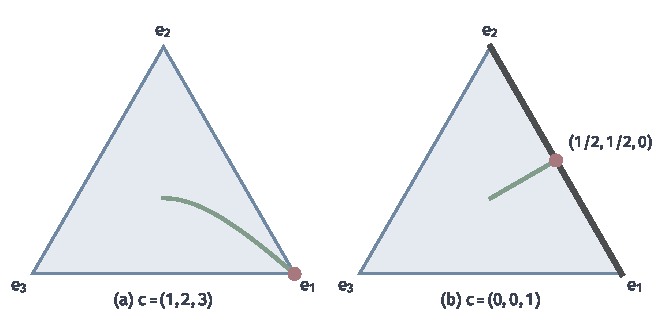
\includegraphics[width=112mm]{figures/05-optimization/01-linear-programming/matplotlib/lpipm-optimal-face/figure.pdf}
  \caption{路径的极限由最优解集决定。绿线是中心路径。(a)$\bm{c}=(1,2,3)$，最优解唯一，路径通向顶点$\bm{e}_1$（红点）。(b)$\bm{c}=(0,0,1)$，最优解集是深灰粗线表示的整条边，路径通向这条边的中点$(1/2,1/2,0)^\top$，这是最优面上的解析中心，不是顶点。}
  \label{fig:lpipm-optimal-face}
\end{BookInlineFigure}

一般情形的结论如下。设最优解集合为$\bm{S}_{\mathrm{P}}$，这是可行集的一个面，称为\term{最优面}（optimal face）。若某对原始、对偶最优解满足对每个下标$x_i^\star+s_i^\star>0$，就称这对解是\term{严格互补}（strictly complementary）的。下面的定理说，中心路径收敛到一对严格互补的解，并且在最优面上取在“最中央”的位置。

\begin{theorem}[中心路径的极限]
\label{thm:lpipm-central-limit}
设$\bm{A}$满行秩，$\mathcal{F}^{\circ}$非空。当$\mu\downarrow0$时，$(\bm{x}(\mu),\bm{y}(\mu),\bm{s}(\mu))$收敛到一对最优解$(\hat{\bm{x}},\hat{\bm{y}},\hat{\bm{s}})$。记$B=\{i:\hat{x}_i>0\}$，$N=\{i:\hat{s}_i>0\}$，则$B$与$N$互不相交且并集为$\{1,\ldots,n\}$，并且$\hat{\bm{x}}$是最优面上使下式最大的唯一点：
\begin{equation}
 \sum_{i\in B}\log x_i.
 \label{eq:lpipm-face-center}
\end{equation}
\end{theorem}

\begin{proof}
关键工具是一个正交关系。设$\bm{x},\bm{x}'$都满足等式$\bm{A}\bm{x}=\bm{b}$，$(\bm{y},\bm{s}),(\bm{y}',\bm{s}')$都满足$\bm{A}^\top\bm{y}+\bm{s}=\bm{c}$。则$\bm{x}-\bm{x}'$属于$\bm{A}$的零空间，$\bm{s}-\bm{s}'=-\bm{A}^\top(\bm{y}-\bm{y}')$属于$\bm{A}^\top$的列空间，于是
\begin{equation}
 (\bm{x}-\bm{x}')^\top(\bm{s}-\bm{s}')=0.
 \label{eq:lpipm-orthogonality}
\end{equation}

\emph{有界性。}取固定的$(\bar{\bm{x}},\bar{\bm{y}},\bar{\bm{s}})\in\mathcal{F}^{\circ}$。把式~\eqref{eq:lpipm-orthogonality}用到中心点和这一点，展开并用$\bm{x}(\mu)^\top\bm{s}(\mu)=n\mu$，得到
\[
 \bar{\bm{s}}^\top\bm{x}(\mu)+\bar{\bm{x}}^\top\bm{s}(\mu)=n\mu+\bar{\bm{x}}^\top\bar{\bm{s}}.
\]
左边各项非负且$\bar{\bm{x}},\bar{\bm{s}}>\bm{0}$，所以$\mu\in(0,1]$时$\bm{x}(\mu)$、$\bm{s}(\mu)$有界。$\bm{A}^\top$列满秩，$\bm{y}(\mu)$也有界。

\emph{聚点是最优解。}取$\mu_k\downarrow0$使三元组收敛到一个聚点$(\hat{\bm{x}},\hat{\bm{y}},\hat{\bm{s}})$。它满足两组等式，$\hat{\bm{x}},\hat{\bm{s}}\geq\bm{0}$，且由式~\eqref{eq:lpipm-central-gap}，$\hat{\bm{x}}^\top\hat{\bm{s}}=0$，所以是最优解。

\emph{一个归一化的恒等式。}设$(\bm{x}^\star,\bm{y}^\star,\bm{s}^\star)$是任意一对最优解，由互补松弛，它们的内积为零。把式~\eqref{eq:lpipm-orthogonality}用到中心点和这一对最优解，得到
\[
 (\bm{s}^\star)^\top\bm{x}(\mu)+(\bm{x}^\star)^\top\bm{s}(\mu)=n\mu.
\]
两边除以$\mu$，用$x_i(\mu)/\mu=1/s_i(\mu)$和$s_i(\mu)/\mu=1/x_i(\mu)$，得到
\begin{equation}
 \sum_{i=1}^n\frac{s_i^\star}{s_i(\mu)}+\sum_{i=1}^n\frac{x_i^\star}{x_i(\mu)}=n.
 \label{eq:lpipm-normalized}
\end{equation}

\emph{严格互补。}式~\eqref{eq:lpipm-normalized}左边每一项非负，所以$x_i(\mu)\geq x_i^\star/n$。令$\mu=\mu_k\to0$，得$\hat{x}_i\geq x_i^\star/n$，即每个最优解的正分量也是$\hat{\bm{x}}$的正分量；对$\hat{\bm{s}}$同理。

再把聚点$(\hat{\bm{x}},\hat{\bm{s}})$本身当作最优解代入式~\eqref{eq:lpipm-normalized}，令$\mu_k\to0$。$i\in B$时$\hat{x}_i/x_i(\mu_k)\to1$，$i\in N$时$\hat{s}_i/s_i(\mu_k)\to1$，其余项为零，于是
\[
 \lvert B\rvert+\lvert N\rvert=n.
\]
互补性$\hat{\bm{x}}^\top\hat{\bm{s}}=0$说明$B\cap N=\varnothing$，所以它们的并集是全部下标。

\emph{极限唯一。}由上一步，任何聚点的正分量位置都包含任何最优解的正分量位置，所以所有聚点有相同的$B$和$N$，任何原始最优解在$N$上为零。在式~\eqref{eq:lpipm-normalized}中取$\bm{s}^\star=\hat{\bm{s}}$、$\bm{x}^\star$为任意原始最优解，令$\mu_k\to0$，得到
\[
 \lvert N\rvert+\sum_{i\in B}\frac{x_i^\star}{\hat{x}_i}=n,\qquad\text{即}\qquad\sum_{i\in B}\frac{x_i^\star-\hat{x}_i}{\hat{x}_i}=0.
\]
这正是凹函数~\eqref{eq:lpipm-face-center}在$\hat{\bm{x}}$处沿任意最优面方向的方向导数为零，所以$\hat{\bm{x}}$是它在最优面上的最大点。严格凹性保证最大点唯一，因此所有聚点的$\bm{x}$部分相同。对$\hat{\bm{s}}$同理，得到相应的$\sum_{i\in N}\log s_i$最大的唯一点，再由$\bm{A}^\top$列满秩，$\hat{\bm{y}}$也唯一。有界序列只有一个聚点，所以收敛。
\end{proof}

这个定理有两个直接的推论。最优解唯一时，路径通向顶点；最优解不唯一时，路径通向最优面的相对内部，得不到顶点。此外，定理顺带证明了线性规划在$\mathcal{F}^{\circ}$非空时总有严格互补解。

这里的下标集$B$和单纯形法的基不是一回事：$B$是极限点的正分量位置，可以多于或少于$m$个。内点法最终告诉我们的是“哪些变量为正”，而不是直接给出一个基，第~\ref{sec:lpipm-accuracy}节会处理两者的转换。

\section{原始—对偶路径跟踪}
\label{sec:lpipm-path-following}

上一节得到一条曲线，但求曲线上的一个点要解一组非线性方程。于是要问：不把每个中心点算准，怎样一步步沿曲线走向$\mu=0$？做法是把三组条件当作一个方程组，同时更新$\bm{x},\bm{y},\bm{s}$。

\paragraph{主要思想：对扰动方程作Newton线性化}
当前点记为$(\bm{x},\bm{y},\bm{s})$，只要求$\bm{x},\bm{s}>\bm{0}$。为了同时适用下一节的不可行起点，这里不假设它满足等式约束。当前的平均互补量是
\begin{equation}
 \mu=\frac{\bm{x}^\top\bm{s}}{n}.
 \label{eq:lpipm-mu}
\end{equation}

我们不把目标定为$\mu=0$，而定为路径上$\sigma\mu$处的中心点，其中$\sigma\in[0,1]$称为\term{中心化参数}（centering parameter）。这一轮想达到的是
\[
 \bm{A}\bm{x}=\bm{b},\qquad\bm{A}^\top\bm{y}+\bm{s}=\bm{c},\qquad x_is_i=\sigma\mu.
\]

把新的点写成$\bm{x}+\Delta\bm{x}$、$\bm{y}+\Delta\bm{y}$、$\bm{s}+\Delta\bm{s}$，代入这三组方程。前两组本身就是线性的，第三组展开是
\[
 x_is_i+s_i\Delta x_i+x_i\Delta s_i+\Delta x_i\Delta s_i=\sigma\mu.
\]
唯一的非线性项是$\Delta x_i\Delta s_i$，它是两个小量的乘积。Newton法的做法就是把它丢掉，留下关于方向的线性方程组。

为了写得紧凑，定义三个残差，分别度量原始等式、对偶等式和互补目标还差多少：
\begin{equation}
 \bm{r}_{\mathrm{p}}=\bm{A}\bm{x}-\bm{b},\qquad
 \bm{r}_{\mathrm{d}}=\bm{A}^\top\bm{y}+\bm{s}-\bm{c},\qquad
 \bm{r}_{\mathrm{c}}=\sigma\mu\bm{1}-\bm{X}\bm{S}\bm{1},
 \label{eq:lpipm-residuals}
\end{equation}
其中$\bm{S}=\operatorname{diag}(\bm{s})$。这样，方向$(\Delta\bm{x},\Delta\bm{y},\Delta\bm{s})$由下面的线性方程组确定：
\begin{equation}
 \begin{bmatrix}
 \bm{A}&\bm{0}&\bm{0}\\
 \bm{0}&\bm{A}^\top&\bm{I}\\
 \bm{S}&\bm{0}&\bm{X}
 \end{bmatrix}
 \begin{bmatrix}\Delta\bm{x}\\\Delta\bm{y}\\\Delta\bm{s}\end{bmatrix}
 =
 \begin{bmatrix}-\bm{r}_{\mathrm{p}}\\-\bm{r}_{\mathrm{d}}\\\bm{r}_{\mathrm{c}}\end{bmatrix}.
 \label{eq:lpipm-newton}
\end{equation}
第一行要求走完之后原始残差消失，第二行要求对偶残差消失，第三行要求所有乘积都变成$\sigma\mu$。系数矩阵正是三组方程关于$(\bm{x},\bm{y},\bm{s})$的Jacobian矩阵。

\paragraph{为什么线性化$x_is_i=\mu$，而不是$s_i=\mu/x_i$}
两种写法定义同一条曲线，线性化后的方程却差别很大。图~\ref{fig:lpipm-newton-bilinear}取一个坐标，固定$s=1$、$\mu=1$，方程的根是$x=1$。图(a)对$\mu/x-s=0$作Newton法，从$x=2.4$出发，切线与横轴的交点落在$x\approx-0.96$，越过了边界。

这件事不是偶然的。$1/x$在$x$大时很平，切线斜率过小，步子迈得过大；具体地，这个迭代是$x\mapsto x(2-x)$，$x>2$时一步变成负数。图(b)对$xs-\mu=0$作Newton法，函数本身关于$x$是直线，一步到根。一般情形中$s$也在变，方程对两个变量合起来是双线性的，但误差只是一个二阶小项$\Delta x_i\Delta s_i$，线性模型“可信的范围”比倒数形式大得多。

\begin{BookInlineFigure}
  \centering
  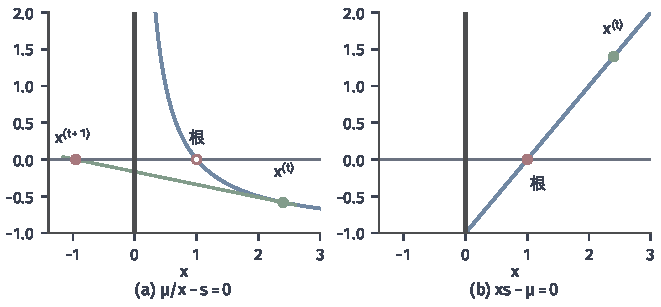
\includegraphics[width=112mm]{figures/05-optimization/01-linear-programming/matplotlib/lpipm-newton-bilinear/figure.pdf}
  \caption{同一条约束的两种写法，$s=\mu=1$，根都是$x=1$（红圈或红点）。(a)蓝线是$\mu/x-s$，绿线是在$x^{(t)}=2.4$处的切线，Newton步落到$x^{(t+1)}\approx-0.96$（红点），越过边界（深灰粗线）。(b)蓝线是$xs-\mu$，本身就是直线，Newton步一步到根。}
  \label{fig:lpipm-newton-bilinear}
\end{BookInlineFigure}

\paragraph{消元：把方程组化成一个$m\times m$的问题}
方程组~\eqref{eq:lpipm-newton}的大小是$2n+m$，但结构很特殊，可以依次消元。由第二行，
\begin{equation}
 \Delta\bm{s}=-\bm{r}_{\mathrm{d}}-\bm{A}^\top\Delta\bm{y}.
 \label{eq:lpipm-ds}
\end{equation}
第三行是$\bm{S}$与$\bm{X}$两个对角矩阵分别作用在两个方向上，直接解出
\begin{equation}
 \Delta\bm{x}=\bm{S}^{-1}\bigl(\bm{r}_{\mathrm{c}}-\bm{X}\Delta\bm{s}\bigr).
 \label{eq:lpipm-dx}
\end{equation}
把式~\eqref{eq:lpipm-ds}代入式~\eqref{eq:lpipm-dx}，得到
\[
 \Delta\bm{x}=\bm{S}^{-1}\bigl(\bm{r}_{\mathrm{c}}+\bm{X}\bm{r}_{\mathrm{d}}\bigr)+\bm{S}^{-1}\bm{X}\bm{A}^\top\Delta\bm{y}.
\]

记对角矩阵$\bm{D}=\bm{X}\bm{S}^{-1}$，它的对角元是$x_i/s_i$。把上式代入第一行$\bm{A}\Delta\bm{x}=-\bm{r}_{\mathrm{p}}$，就得到只含$\Delta\bm{y}$的方程。定义
\begin{equation}
 \bm{M}=\bm{A}\bm{D}\bm{A}^\top,\qquad
 \bm{h}=-\bm{r}_{\mathrm{p}}-\bm{A}\bm{S}^{-1}\bigl(\bm{r}_{\mathrm{c}}+\bm{X}\bm{r}_{\mathrm{d}}\bigr),
 \label{eq:lpipm-normal-data}
\end{equation}
方向$\Delta\bm{y}$由下式给出：
\begin{equation}
 \Delta\bm{y}=\bm{M}^{-1}\bm{h}.
 \label{eq:lpipm-dy}
\end{equation}
$\bm{M}\Delta\bm{y}=\bm{h}$称为\term{正规方程}（normal equations），实际计算中用Cholesky分解求解，不显式求逆。求出$\Delta\bm{y}$后，由式~\eqref{eq:lpipm-ds}得到$\Delta\bm{s}$，再由式~\eqref{eq:lpipm-dx}得到$\Delta\bm{x}$。

这一步之所以总能进行，靠的是下面的事实。

\begin{lemma}[Newton方程可解]
\label{lem:lpipm-newton-solvable}
设$\bm{A}$满行秩，$\bm{x},\bm{s}>\bm{0}$。则$\bm{M}=\bm{A}\bm{D}\bm{A}^\top$对称正定，方程组~\eqref{eq:lpipm-newton}有唯一解，由式~\eqref{eq:lpipm-dy}、\eqref{eq:lpipm-ds}、\eqref{eq:lpipm-dx}给出。
\end{lemma}

\begin{proof}
$\bm{D}$的对角元全为正。对任何$\bm{v}\neq\bm{0}$，$\bm{A}$满行秩给出$\bm{A}^\top\bm{v}\neq\bm{0}$，于是
\[
 \bm{v}^\top\bm{M}\bm{v}=(\bm{A}^\top\bm{v})^\top\bm{D}(\bm{A}^\top\bm{v})>0,
\]
所以$\bm{M}$正定。上面的消元每一步都是等价变形，故方程组的解恰好由这三个公式给出。
\end{proof}

\paragraph{一步之后三个残差怎样变}
设步长为$\alpha\in(0,1]$，$\bm{x}^+=\bm{x}+\alpha\Delta\bm{x}$，$\bm{y}^+$、$\bm{s}^+$同理。前两组方程是线性的，把第一行、第二行代入，新的残差就是
\begin{equation}
 \bm{r}_{\mathrm{p}}^+=(1-\alpha)\bm{r}_{\mathrm{p}},\qquad\bm{r}_{\mathrm{d}}^+=(1-\alpha)\bm{r}_{\mathrm{d}}.
 \label{eq:lpipm-residual-update}
\end{equation}
走完单位步（$\alpha=1$）时，等式残差恰好为零，此后一直为零。

互补量的变化由展开式得到。把$\bm{x}^+$、$\bm{s}^+$代入内积，一次项由第三行给出
\[
 \bm{s}^\top\Delta\bm{x}+\bm{x}^\top\Delta\bm{s}=\bm{1}^\top\bm{r}_{\mathrm{c}}=n\sigma\mu-n\mu,
\]
于是
\begin{equation}
 (\bm{x}^+)^\top\bm{s}^+=\bigl(1-\alpha(1-\sigma)\bigr)\bm{x}^\top\bm{s}+\alpha^2\,\Delta\bm{x}^\top\Delta\bm{s}.
 \label{eq:lpipm-comp-update}
\end{equation}
当前点严格可行时，两个等式残差为零，第一行和第二行给出
\[
 \bm{A}\Delta\bm{x}=\bm{0},\qquad\Delta\bm{s}=-\bm{A}^\top\Delta\bm{y}.
\]
所以$\Delta\bm{x}^\top\Delta\bm{s}=0$，互补量精确地按因子$1-\alpha(1-\sigma)$下降。

\paragraph{步长：到边界的比例}
Newton方向可能把某个分量推成负数，所以步长要受限。沿方向走时，每个正分量到零的距离是确定的。定义能保持非负的最大步长
\begin{equation}
 \alpha_{\max}=\min\Bigl\{\min_{\Delta x_i<0}\frac{x_i}{-\Delta x_i},\ \min_{\Delta s_i<0}\frac{s_i}{-\Delta s_i}\Bigr\},
 \label{eq:lpipm-alpha-max}
\end{equation}
没有负分量时约定$\alpha_{\max}=+\infty$。这个量和单纯形法的比值检验是同一种计算，只是后者走到恰好有一个变量为零，这里不能走到那么远，否则下一轮的$\bm{S}^{-1}$或$\bm{D}$不存在。

取一个略小于$1$的比例$\eta$，例如$0.9$或$0.995$，令
\begin{equation}
 \alpha=\min\{1,\ \eta\,\alpha_{\max}\},
 \label{eq:lpipm-alpha}
\end{equation}
这称为\term{到边界的比例规则}（fraction-to-the-boundary rule）。图~\ref{fig:lpipm-step-rule}是贯穿例第一轮的情形：六个坐标沿方向变化，其中$s_1$最先降到零，$\alpha_{\max}$由它决定。

\begin{BookInlineFigure}
  \centering
  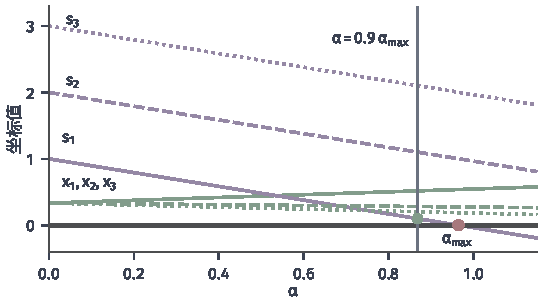
\includegraphics[width=92mm]{figures/05-optimization/01-linear-programming/matplotlib/lpipm-step-rule/figure.pdf}
  \caption{贯穿例第一轮各坐标沿Newton方向的变化，$\sigma=0.3$。紫线是$s_1,s_2,s_3$，绿线是$x_1,x_2,x_3$，实线、虚线、点线依次对应下标$1,2,3$，深灰粗线是边界。$s_1$在$\alpha_{\max}=55/57\approx0.965$处最先到达零（红点），取$\eta=0.9$后实际步长$\alpha=33/38\approx0.868$（竖线与绿点）。}
  \label{fig:lpipm-step-rule}
\end{BookInlineFigure}

\paragraph{中心化：两种力量的折中}
参数$\sigma$控制这一轮更想做什么。$\sigma=1$时目标是当前$\mu$处的中心点，方向只把点拉回路径，互补量不减；$\sigma=0$时目标直接是$\mu=0$，这个方向称为\term{仿射尺度方向}（affine-scaling direction），只求减小互补量，不管中心性。

可以把中心路径想成山谷的谷线，互补量是海拔。$\sigma=0$相当于只顾朝谷底方向走，容易撞上谷壁，步长被迫很小。$\sigma=1$相当于退回谷线，位置好了，海拔没降。合适的$\sigma$介于两者之间，类比的失效之处是，这里“谷壁”是$x_i$或$s_i$接近零的边界，不是某个目标函数的等高线。

\paragraph{计算过程}
下面把每一轮写成具体步骤，并在例~\eqref{eq:lpipm-running}上逐轮计算。取固定的中心化参数$\sigma=0.3$、比例$\eta=0.9$，容差$\varepsilon=10^{-3}$，起点选严格可行点。

\needspace{6\baselineskip}
\paragraph{变量}
\begin{itemize}
 \item $\bm{x}\in\mathbb{R}^n$：当前原始点，所有分量为正。
 \item $\bm{y}\in\mathbb{R}^m$：当前对偶变量。
 \item $\bm{s}\in\mathbb{R}^n$：当前对偶松弛，所有分量为正。
 \item $\mu$：当前平均互补量，由式~\eqref{eq:lpipm-mu}计算。
 \item $\bm{r}_{\mathrm{p}},\bm{r}_{\mathrm{d}},\bm{r}_{\mathrm{c}}$：式~\eqref{eq:lpipm-residuals}的三个残差，形状分别是$m$、$n$、$n$维。
 \item $\bm{D}$、$\bm{M}$、$\bm{h}$：对角缩放矩阵、$m\times m$的正规矩阵和右端，由式~\eqref{eq:lpipm-normal-data}计算。
 \item $\Delta\bm{x},\Delta\bm{y},\Delta\bm{s}$：本轮的方向，$\alpha_{\max},\alpha$是最大步长和实际步长。
\end{itemize}

\paragraph{初始化}
取严格可行的起点$(\bm{x}^{(0)},\bm{y}^{(0)},\bm{s}^{(0)})\in\mathcal{F}^{\circ}$，令$t=0$；起点怎样得到由下一节回答。例中取
\[
 \bm{x}^{(0)}=\Bigl(\frac13,\frac13,\frac13\Bigr)^\top,\qquad y^{(0)}=0,\qquad\bm{s}^{(0)}=(1,2,3)^\top.
\]
它满足等式约束，但不是中心点：三个乘积分别是$1/3$、$2/3$、$1$。

\needspace{6\baselineskip}
\paragraph{每轮更新}
在第$t$轮，以$(\bm{x}^{(t)},\bm{y}^{(t)},\bm{s}^{(t)})$为当前点：
\begin{enumerate}
 \item \textbf{检查停止。}按式~\eqref{eq:lpipm-residuals}计算$\bm{r}_{\mathrm{p}}$、$\bm{r}_{\mathrm{d}}$，按式~\eqref{eq:lpipm-mu}计算$\mu^{(t)}$。若等式残差和互补量都不超过容差，停止并输出当前点。

 例中第一轮
 \[
  \mu^{(0)}=\frac13\Bigl(\frac13+\frac23+1\Bigr)=\frac23,\qquad\bm{x}^\top\bm{s}=2>\varepsilon,
 \]
 等式残差都是零，继续。

 \item \textbf{计算互补残差。}按式~\eqref{eq:lpipm-residuals}计算$\bm{r}_{\mathrm{c}}$，这里的$\mu$取$\mu^{(t)}$。

 例中第一轮$\sigma\mu^{(0)}=1/5$，
 \[
  \bm{r}_{\mathrm{c}}=\frac15\bm{1}-\Bigl(\frac13,\frac23,1\Bigr)^\top=\Bigl(-\frac{2}{15},-\frac{7}{15},-\frac45\Bigr)^\top.
 \]

 \item \textbf{形成并求解正规方程。}由式~\eqref{eq:lpipm-normal-data}计算$\bm{M}$和$\bm{h}$，由式~\eqref{eq:lpipm-dy}得到$\Delta\bm{y}$。

 例中$\bm{r}_{\mathrm{p}},\bm{r}_{\mathrm{d}}$为零，$\bm{D}$的对角元是$x_i/s_i$，$\bm{A}$是一行全一，所以$\bm{M}$和$\bm{h}$都是数。第一轮
 \[
  M=\frac13+\frac16+\frac19=\frac{11}{18},\qquad h=-\sum_{i=1}^3\frac{r_{\mathrm{c},i}}{s_i}=\frac{2}{15}+\frac{7}{30}+\frac{4}{15}=\frac{19}{30},
 \]
 于是
 \[
  \Delta y=\frac{19/30}{11/18}=\frac{57}{55}\approx1.0364.
 \]

 \item \textbf{回代方向。}由式~\eqref{eq:lpipm-ds}得到$\Delta\bm{s}$，由式~\eqref{eq:lpipm-dx}得到$\Delta\bm{x}$。

 例中第一轮$\Delta\bm{s}=-\Delta y\bm{1}$，$\Delta x_i=(r_{\mathrm{c},i}-x_i\Delta s_i)/s_i$，于是
 \[
  \Delta\bm{s}=-\frac{57}{55}\bm{1},\qquad
  \Delta\bm{x}=\Bigl(\frac{7}{33},-\frac{2}{33},-\frac{5}{33}\Bigr)^\top.
 \]
 三个$\Delta x_i$相加为零，这正是$\bm{A}\Delta\bm{x}=\bm{0}$。

 \item \textbf{确定步长。}由式~\eqref{eq:lpipm-alpha-max}、\eqref{eq:lpipm-alpha}计算$\alpha_{\max}$和$\alpha$。

 例中第一轮三个$s_i$的比值分别是$\tfrac{55}{57},\tfrac{110}{57},\tfrac{165}{57}$，$x_2,x_3$的比值分别是$\tfrac{11}{2},\tfrac{11}{5}$，最小的是$s_1$的比值，所以
 \[
  \alpha_{\max}=\frac{55}{57}\approx0.9649,\qquad\alpha=\frac{9}{10}\cdot\frac{55}{57}=\frac{33}{38}\approx0.8684.
 \]

 \item \textbf{更新。}令
 \begin{equation}
  \begin{aligned}
  \bm{x}^{(t+1)}&=\bm{x}^{(t)}+\alpha\Delta\bm{x},\\
  \bm{y}^{(t+1)}&=\bm{y}^{(t)}+\alpha\Delta\bm{y},\\
  \bm{s}^{(t+1)}&=\bm{s}^{(t)}+\alpha\Delta\bm{s},
  \end{aligned}
  \label{eq:lpipm-update}
 \end{equation}
 然后令$t\leftarrow t+1$，回到第1步。这里原始变量和对偶变量用同一个步长，式~\eqref{eq:lpipm-comp-update}的精确下降公式依赖这一点。

 例中第一轮
 \[
  \bm{x}^{(1)}=\Bigl(\frac{59}{114},\frac{16}{57},\frac{23}{114}\Bigr)^\top\approx(0.5175,0.2807,0.2018)^\top,
 \]
 对偶部分是
 \[
  y^{(1)}=\frac{9}{10},\qquad\bm{s}^{(1)}=\Bigl(\frac{1}{10},\frac{11}{10},\frac{21}{10}\Bigr)^\top.
 \]
 按式~\eqref{eq:lpipm-comp-update}，互补量应是
 \[
  \Bigl(1-\frac{33}{38}\cdot\frac{7}{10}\Bigr)\cdot2=\frac{149}{190}\approx0.7842.
 \]
 直接计算$\sum_ix_i^{(1)}s_i^{(1)}$也得到这个数。

 三个乘积这时是$(0.0518,0.3088,0.4237)$，差距比起点时大了，这一步以中心性为代价换来了较长的步子。
\end{enumerate}

例中第二轮的中间量如下。当前$\mu^{(1)}=0.2614$，$\sigma\mu^{(1)}=0.07842$，
\[
 \begin{gathered}
 \bm{r}_{\mathrm{c}}=(0.0267,-0.2304,-0.3453)^\top,\\
 \bm{D}=\operatorname{diag}(5.1754,0.2552,0.0961).
 \end{gathered}
\]
第一个分量已经被压低，$x_1s_1$小于目标$\sigma\mu$，所以$r_{\mathrm{c},1}$变成正的，这一轮要把它往上拉。

正规方程给出
\[
 M=5.5267,\qquad h=0.1072,\qquad\Delta y=0.0194.
\]
回代得到
\[
 \Delta\bm{s}=-0.0194\,\bm{1},\qquad\Delta\bm{x}=(0.3670,-0.2045,-0.1625)^\top.
\]

这一轮$\alpha_{\max}=1.2412$，$0.9\alpha_{\max}>1$，所以取$\alpha=1$，于是
\[
 \begin{gathered}
 \bm{x}^{(2)}=(0.8846,0.0762,0.0392)^\top,\qquad y^{(2)}=0.9194,\\
 \bm{s}^{(2)}=(0.0806,1.0806,2.0806)^\top.
 \end{gathered}
\]
互补量精确地变为$0.3\times0.7842=0.2353$。

此后每轮都取$\alpha=1$，互补量每轮乘以$0.3$。表~\ref{tab:lpipm-run}列出全部$7$轮的中间量。第$7$轮后互补量约为$5.7\times10^{-4}$，不超过$\varepsilon$，算法停止。

\begin{BookInlineTable}
  \centering
  \footnotesize
  \begin{tabular}{@{}ccccccccc@{}}
    \toprule
    $t$ & $x_1^{(t)}$ & $x_2^{(t)}$ & $y^{(t)}$ & $\mu^{(t)}$ & $M$ & $\Delta y$ & $\alpha_{\max}$ & $\alpha$\\
    \midrule
    0 & 0.3333 & 0.3333 & 0 & 0.6667 & 0.6111 & 1.0364 & 0.9649 & 0.8684\\
    1 & 0.5175 & 0.2807 & 0.9 & 0.2614 & 5.527 & 0.0194 & 1.2412 & 1\\
    2 & 0.8846 & 0.0762 & 0.9194 & 0.0784 & 11.06 & 0.0610 & 1.3210 & 1\\
    3 & 0.9615 & 0.0261 & 0.9804 & 0.0235 & 49.12 & 0.0128 & 1.3851 & 1\\
    4 & 0.9892 & 0.0073 & 0.9932 & 0.0071 & 146.0 & 0.0047 & 1.4179 & 1\\
    5 & 0.9968 & 0.0021 & 0.9979 & 0.0021 & 477.3 & 0.0015 & 1.4247 & 1\\
    6 & 0.9990 & 0.0006 & 0.9994 & 0.0006 & 1579 & 0.0004 & 1.4274 & 1\\
    7 & 0.9997 & 0.0002 & 0.9998 & 0.0002 & & & & \\
    \bottomrule
  \end{tabular}
  \caption{贯穿例的逐轮中间量，$\sigma=0.3$、$\eta=0.9$。$x_3^{(t)}=1-x_1^{(t)}-x_2^{(t)}$，$s_i^{(t)}=c_i-y^{(t)}$。第$t$行的$M,\Delta y,\alpha_{\max},\alpha$是从第$t$个点出发那一轮的量。}
  \label{tab:lpipm-run}
\end{BookInlineTable}

最终得到
\[
 \hat{\bm{x}}\approx(0.9997,0.0002,0.0001)^\top,\qquad\hat{y}\approx0.9998,
\]
互补量约$5.7\times10^{-4}$，目标值$\bm{c}^\top\hat{\bm{x}}\approx1.0004$。由于迭代全程可行，间隙就是互补量，目标误差不超过$5.7\times10^{-4}$。实际误差约$3.8\times10^{-4}$，确实在这个界内。这里的$\hat{\bm{x}}$不是顶点，第~\ref{sec:lpipm-accuracy}节讨论这一点的影响。

\begin{BookInlineFigure}
  \centering
  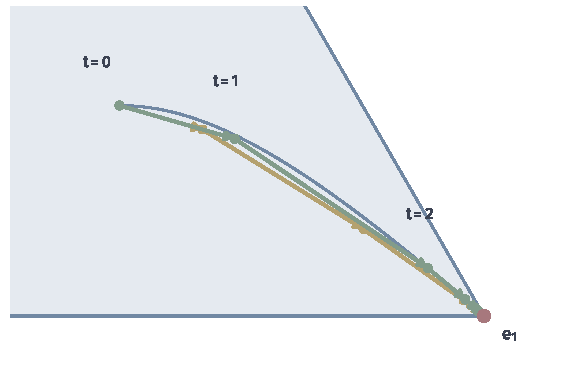
\includegraphics[width=96mm]{figures/05-optimization/01-linear-programming/matplotlib/lpipm-iterates/figure.pdf}
  \caption{贯穿例的迭代点，三角形局部放大。蓝线是中心路径，绿色是$\sigma=0.3$的路径跟踪，黄色是更激进的$\sigma=0.1$，红点是最优顶点$\bm{e}_1$。迭代点不在路径上，而是绕在路径附近前进。}
  \label{fig:lpipm-iterates}
\end{BookInlineFigure}

\paragraph{$\sigma$的取值}
图~\ref{fig:lpipm-iterates}中迭代点没有贴着路径，但始终在它附近。这种“附近”的程度可以用$\min_ix_is_i/\mu$度量，它等于$1$时点是中心点，接近$0$时某个乘积远低于平均。

图~\ref{fig:lpipm-sigma-tradeoff}比较了不同的$\sigma$。图(a)中，$\sigma$越小，互补量下降越快，但这只是因为每轮的目标更激进。图(b)说明了代价：$\sigma=0.1$前两轮的步长只有$0.63$和$0.68$，到$t=2$时中心性掉到$0.07$左右，靠后面的几轮才恢复。$\sigma=0.9$则一直很靠近中心，下降却极慢。

\begin{BookInlineFigure}
  \centering
  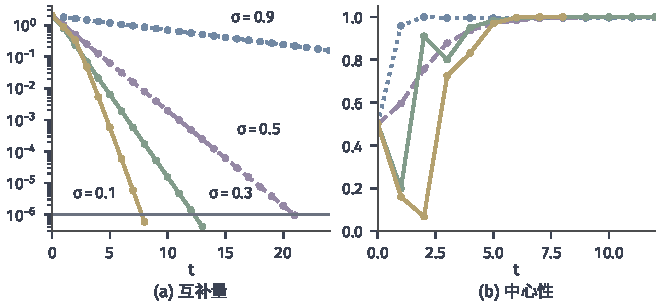
\includegraphics[width=112mm]{figures/05-optimization/01-linear-programming/matplotlib/lpipm-sigma-tradeoff/figure.pdf}
  \caption{中心化参数的影响，贯穿例，$\eta=0.9$。(a)互补量$\bm{x}^\top\bm{s}$随轮次的变化，灰色横线是$10^{-6}$。(b)中心性$\min_ix_is_i/\mu$，等于$1$表示恰好在中心路径上。绿线$\sigma=0.3$，黄线$\sigma=0.1$，紫色虚线$\sigma=0.5$，蓝色点线$\sigma=0.9$。}
  \label{fig:lpipm-sigma-tradeoff}
\end{BookInlineFigure}

\paragraph{预测—校正：先试走一步}
固定的$\sigma$有两个缺点：它不知道这一轮能走多远，也没有处理被丢掉的二阶项$\Delta x_i\Delta s_i$。\term{预测—校正}（predictor-corrector）方法用一次试算解决这两件事，额外代价只是多解一次已经分解好的方程组。

\emph{预测}是先解一次$\sigma=0$的方程组，得到仿射尺度方向$(\Delta\bm{x}^{\mathrm{a}},\Delta\bm{y}^{\mathrm{a}},\Delta\bm{s}^{\mathrm{a}})$，也就是令$\bm{r}_{\mathrm{c}}=-\bm{X}\bm{S}\bm{1}$。沿它能走的步长记为$\alpha^{\mathrm{a}}$，试走之后的平均互补量是
\begin{equation}
 \mu^{\mathrm{a}}=\frac{(\bm{x}+\alpha^{\mathrm{a}}\Delta\bm{x}^{\mathrm{a}})^\top(\bm{s}+\alpha^{\mathrm{a}}\Delta\bm{s}^{\mathrm{a}})}{n}.
 \label{eq:lpipm-mu-aff}
\end{equation}

这个数说明当前点有多好走：$\mu^{\mathrm{a}}$远小于$\mu$时，纯下降方向很有效，不需要多少中心化。常用的选法是
\begin{equation}
 \sigma=\Bigl(\frac{\mu^{\mathrm{a}}}{\mu}\Bigr)^3.
 \label{eq:lpipm-sigma-rule}
\end{equation}
三次方是一条经验规则，没有理论上的必然性。

\emph{校正}处理二阶项。式~\eqref{eq:lpipm-newton}假装$\Delta x_i\Delta s_i=0$，预测步已经给出了这一项的估计$\Delta x_i^{\mathrm{a}}\Delta s_i^{\mathrm{a}}$，于是把它移到右端：
\begin{equation}
 \bm{r}_{\mathrm{c}}=\sigma\mu\bm{1}-\bm{X}\bm{S}\bm{1}-\Delta\bm{X}^{\mathrm{a}}\Delta\bm{S}^{\mathrm{a}}\bm{1}.
 \label{eq:lpipm-corrector-rhs}
\end{equation}
用这个$\bm{r}_{\mathrm{c}}$按式~\eqref{eq:lpipm-normal-data}至\eqref{eq:lpipm-dx}求方向，步长仍按式~\eqref{eq:lpipm-alpha}。两次求解的系数矩阵$\bm{M}$相同，所以只分解一次，这一点在$\bm{M}$很大时决定了这个方法的价值。

例中第一轮，预测方向取$\sigma=0$，$M$与前面相同，右端变成$h=1$，得到
\[
 \Delta y^{\mathrm{a}}=\frac{18}{11},\qquad\Delta\bm{x}^{\mathrm{a}}=\Bigl(\frac{7}{33},-\frac{2}{33},-\frac{5}{33}\Bigr)^\top.
\]
这里$\Delta\bm{x}^{\mathrm{a}}$与固定$\sigma=0.3$时相同，是因为起点是三角形的解析中心，中心化分量在$\bm{x}$上恰好为零。

步长由$s_1$决定，试走后的互补量和中心化参数是
\[
 \alpha^{\mathrm{a}}=\frac{11}{18},\qquad\mu^{\mathrm{a}}=\frac{7}{27}\approx0.2593,\qquad\sigma=\Bigl(\frac{7}{18}\Bigr)^3\approx0.0588.
\]

校正的右端由式~\eqref{eq:lpipm-corrector-rhs}算出，其中$\sigma\mu\approx0.0392$，二阶项的估计是
\[
 \Delta\bm{X}^{\mathrm{a}}\Delta\bm{S}^{\mathrm{a}}\bm{1}\approx(-0.3471,0.0992,0.2479)^\top,
\]
于是
\[
 \bm{r}_{\mathrm{c}}\approx(0.0530,-0.7266,-1.2087)^\top,\qquad h\approx0.7132,\qquad\Delta y\approx1.1671.
\]

这一步的最大步长是$\alpha_{\max}\approx0.8568$，取$\alpha\approx0.7711$，得到
\[
 \bm{x}^{(1)}\approx(0.6742,0.2032,0.1226)^\top,\qquad y^{(1)}=0.9,\qquad\bm{x}^\top\bm{s}\approx0.5485.
\]
相比之下，固定$\sigma=0.3$第一轮后的互补量是$0.7842$。

图~\ref{fig:lpipm-predictor-corrector}(a)显示了校正的作用。黄色柱是单位预测步之后的乘积，第一个分量甚至为负，也就是说走完单位步会越界。绿色柱是校正后的单位步，三个乘积都向目标$\sigma\mu$靠拢，虽然这一轮离路径较远，并没有完全到位。

图(b)显示，整体上预测—校正用$7$轮把互补量降到$10^{-6}$以下，固定$\sigma=0.3$用$13$轮。需要说明，这是这个小例子上的观察，式~\eqref{eq:lpipm-sigma-rule}没有迭代次数的一般保证。

\begin{BookInlineFigure}
  \centering
  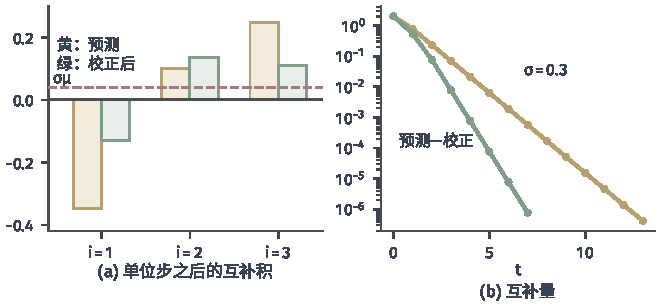
\includegraphics[width=112mm]{figures/05-optimization/01-linear-programming/matplotlib/lpipm-predictor-corrector/figure.pdf}
  \caption{预测—校正的效果，贯穿例。(a)从起点走单位步之后三个乘积$x_is_i$的值：黄色为预测方向，绿色为校正后方向，红色虚线是目标$\sigma\mu\approx0.039$。(b)互补量随轮次的变化，绿线为预测—校正，黄线为固定$\sigma=0.3$，两者都取$\eta=0.9$，容差为$10^{-6}$。}
  \label{fig:lpipm-predictor-corrector}
\end{BookInlineFigure}

\paragraph{计算代价}
每轮的主要工作是形成$\bm{M}=\bm{A}\bm{D}\bm{A}^\top$并作Cholesky分解。稠密情形下，形成$\bm{M}$需要约$m^2n$次运算，分解需要约$m^3/3$次运算；稀疏情形下取决于分解的填充，第~\ref{sec:lpipm-comparison}节再详细讨论。

$\bm{M}$的非零模式只由$\bm{A}$决定，每轮只有$\bm{D}$的数值在变，所以分解的符号结构只需分析一次。回代得到$\Delta\bm{s}$和$\Delta\bm{x}$的代价相对可以忽略。

\section{初始点}
\label{sec:lpipm-initial-point}

上一节的计算从一个严格可行点出发。贯穿例的约束很简单，这样的点一眼可见，一般问题却未必。接下来要弄清：起点从哪里来，起点不可行时算法还能不能用，问题本身没有严格可行点时又该怎么办？

\paragraph{可行初始方法}
最直接的想法是先求出一个严格可行点，再开始路径跟踪，这和单纯形法的第一阶段是同一个思路。对原始一侧，构造辅助问题
\begin{equation}
 \min_{\bm{x},\rho}\ \rho\quad\text{s.t.}\quad\bm{A}\bm{x}=\bm{b},\quad\bm{x}+\rho\bm{1}\geq\bm{0},\quad\rho\geq-1.
 \label{eq:lpipm-phase-one}
\end{equation}
$\rho$越小，$\bm{x}$离边界越有余量。下界$-1$只是为了防止$\rho$在可行集无界时下降到负无穷。

这个辅助问题的严格可行点是现成的：任取$\bm{A}\bm{x}=\bm{b}$的一个解，例如最小范数解$\bm{A}^\top(\bm{A}\bm{A}^\top)^{-1}\bm{b}$，再取足够大的$\rho$即可。最优值$\rho^\star$的符号给出三种结论：

\begin{itemize}
 \item $\rho^\star<0$：最优点满足$x_i\geq-\rho^\star>0$，这是原问题的严格可行点。
 \item $\rho^\star=0$：原问题可行，但没有严格可行点。
 \item $\rho^\star>0$：原问题不可行。
\end{itemize}

三种情形可以用同一个小例子看到。取两个变量和约束$x_1+x_2=a$。把两个分量约束相加，得到$a+2\rho\geq0$，即$\rho\geq-a/2$。取$a=1$时，$\rho^\star=-1/2$，最优点$(1/2,1/2)$严格可行。取$a=0$时，$\rho^\star=0$，可行点只有原点。取$a=-1$时，$\rho^\star=1/2$，原问题不可行。

这个方法有两点不足。辅助问题本身也是线性规划，且它的对偶一侧未必有严格可行点：只有不存在非零的$\bm{d}\geq\bm{0}$使$\bm{A}\bm{d}=\bm{0}$时才有，否则要先加上足够大的变量上界。另外，对偶一侧还要另解一个类似的问题，求出来的点也通常离中心路径很远，要用$\sigma$接近$1$的几步先作中心化。这些原因使大规模实现很少走这条路。

\paragraph{不可行初始方法}
更常用的做法是放弃“起点满足等式”这个要求，只保持$\bm{x},\bm{s}>\bm{0}$。方程组~\eqref{eq:lpipm-newton}的右端本来就含$\bm{r}_{\mathrm{p}}$和$\bm{r}_{\mathrm{d}}$，上一节的公式可以原样使用。式~\eqref{eq:lpipm-residual-update}说明，每走步长$\alpha$，两个等式残差都精确地乘以$1-\alpha$。

这和可行初始方法的区别在于，等式约束不再是“先满足的前提”，而是和互补量一起逐步降低的目标。迭代点在走向最优的同时走向可行。

用贯穿例试算，起点取$\bm{x}^{(0)}=\bm{s}^{(0)}=\bm{1}$、$y^{(0)}=0$，它不满足任何等式。残差是
\[
 r_{\mathrm{p}}=2,\qquad\bm{r}_{\mathrm{d}}=(0,-1,-2)^\top,\qquad\mu^{(0)}=1.
\]
取$\sigma=0.3$，$\bm{r}_{\mathrm{c}}=-0.7\,\bm{1}$。

由式~\eqref{eq:lpipm-normal-data}，$\bm{D}=\bm{I}$，于是
\[
 M=3,\qquad h=-2-\sum_{i=1}^3\bigl(r_{\mathrm{c},i}+r_{\mathrm{d},i}\bigr)=3.1,\qquad\Delta y=\frac{31}{30}\approx1.0333.
\]
回代得到
\[
 \Delta\bm{s}\approx(-1.0333,-0.0333,0.9667)^\top,\qquad\Delta\bm{x}\approx(0.3333,-0.6667,-1.6667)^\top.
\]

$\alpha_{\max}=0.6$由$x_3$决定，取$\alpha=0.54$。新的残差恰好是原来的$0.46$倍，点是
\[
 \bm{x}^{(1)}=(1.18,0.64,0.10)^\top,\qquad y^{(1)}=0.558,\qquad\bm{s}^{(1)}=(0.442,0.982,1.522)^\top.
\]
可以核对$r_{\mathrm{p}}=1.92-1=0.92=0.46\times2$。

接下来第二轮取$\alpha\approx0.894$，第三轮取到$\alpha=1$，等式残差降到舍入误差水平，此后成为可行迭代，如图~\ref{fig:lpipm-infeasible-start}(a)。

\begin{BookInlineFigure}
  \centering
  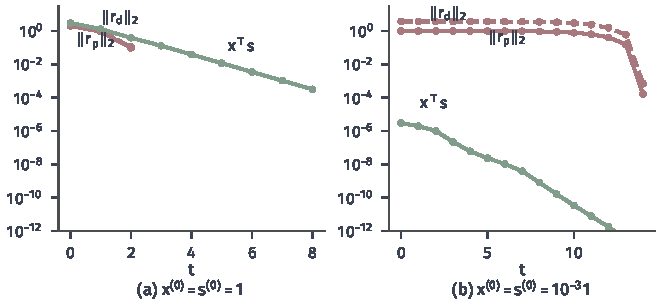
\includegraphics[width=112mm]{figures/05-optimization/01-linear-programming/matplotlib/lpipm-infeasible-start/figure.pdf}
  \caption{不可行起点的两种情况，贯穿例，$\sigma=0.3$、$\eta=0.9$，对数纵轴。红色实线是$\lVert\bm{r}_{\mathrm{p}}\rVert_2$，红色虚线是$\lVert\bm{r}_{\mathrm{d}}\rVert_2$，绿线是$\bm{x}^\top\bm{s}$。(a)起点$\bm{x}=\bm{s}=\bm{1}$，残差在第$3$轮取单位步后归零（图中不再画出）。(b)起点$\bm{x}=\bm{s}=10^{-3}\bm{1}$，互补量先极快地变小，而残差前十轮几乎不动，因为此间的步长只有$10^{-3}$到$10^{-1}$量级。}
  \label{fig:lpipm-infeasible-start}
\end{BookInlineFigure}

\paragraph{起点太小的后果}
图~\ref{fig:lpipm-infeasible-start}(b)把起点缩小到$10^{-3}\bm{1}$。这个起点的互补量已经小到$3\times10^{-6}$，等式残差却仍有$1$和$3.7$的量级。起点小，意味着方程$x_is_i\approx\sigma\mu$的线性化只允许很小的移动：Newton方向要消除大的等式残差，$\alpha_{\max}$却被很小的$x_i,s_i$限制，头几轮的步长只有约$7\times10^{-4}$。

算法最终还是走出来了，但这是这个例子的运气，不是一般保证。理论分析要求互补量不能比等式残差下降得快，常用的条件是
\begin{equation}
 \frac{\lVert(\bm{r}_{\mathrm{p}}^{(t)},\bm{r}_{\mathrm{d}}^{(t)})\rVert_2}{\mu^{(t)}}
 \leq C\,\frac{\lVert(\bm{r}_{\mathrm{p}}^{(0)},\bm{r}_{\mathrm{d}}^{(0)})\rVert_2}{\mu^{(0)}},
 \label{eq:lpipm-infeasible-ratio}
\end{equation}
其中$C\geq1$是常数，并且要求起点足够大。这种算法的全局收敛和复杂度结果需要较长的邻域分析，读者可查阅专著\scite{math-nocedal2006numerical}。在实现中，它对应的经验是起点的$\bm{x}$和$\bm{s}$要足够大，互补量相对残差不能太小。

\paragraph{一个常用的起点}
起点要兼顾两件事：接近满足等式，以及各分量足够大。一个常用的启发式分两步。先求最小范数意义下的近似：
\begin{equation}
 \tilde{\bm{x}}=\bm{A}^\top(\bm{A}\bm{A}^\top)^{-1}\bm{b},\qquad
 \tilde{\bm{y}}=(\bm{A}\bm{A}^\top)^{-1}\bm{A}\bm{c},\qquad
 \tilde{\bm{s}}=\bm{c}-\bm{A}^\top\tilde{\bm{y}}.
 \label{eq:lpipm-mehrotra-start}
\end{equation}
再把负分量和过小的分量整体平移成正的。贯穿例中$\bm{A}\bm{A}^\top=3$，于是$\tilde{\bm{x}}=\tfrac13\bm{1}$，$\tilde{y}=2$，$\tilde{\bm{s}}=(-1,0,1)^\top$。

平移分两步。第一步取$\delta_s=\max\{-1.5\min_i\tilde{s}_i,0\}=1.5$（$\tilde{\bm{x}}$已为正，$\delta_x=0$），得到$\hat{\bm{s}}=(0.5,1.5,2.5)^\top$。第二步按当前互补量再抬高一点，取
\[
 \hat{\delta}_x=\frac12\frac{\tilde{\bm{x}}^\top\hat{\bm{s}}}{\bm{1}^\top\hat{\bm{s}}}=\frac16,\qquad
 \hat{\delta}_s=\frac12\frac{\tilde{\bm{x}}^\top\hat{\bm{s}}}{\bm{1}^\top\tilde{\bm{x}}}=\frac34.
\]
最后的起点是
\[
 \bm{x}^{(0)}=\frac12\bm{1},\qquad y^{(0)}=2,\qquad\bm{s}^{(0)}=(1.25,2.25,3.25)^\top.
\]
这是一条经验规则，没有理论保证，但在实践中通常能避开图~\ref{fig:lpipm-infeasible-start}(b)的情形。

\paragraph{严格可行点不存在时}
定理~\ref{thm:lpipm-central-exists}说明，$\mathcal{F}^{\circ}$为空时中心路径不存在，路径跟踪失去了依据。这种情况有两类来源，处理方式不同。

一类来自建模的表述，问题本身可解。典型例子是把无符号变量写成两个非负变量之差$x=x^+-x^-$：两列互为相反数，第~\ref{sec:lpipm-central-path}节的反例已经说明，这样的问题对偶一侧没有严格可行点。又如约束$x_1+x_2=0$强迫两个变量恒为零。

\term{预处理}（presolve）承担这类任务：删去冗余的行以恢复满行秩，把被约束确定的变量代入，识别恒为零的变量，单独处理自由变量，并把行列缩放到相近的量级。预处理不改变最优解集（或给出恢复原解的办法），却能去掉一大批使严格可行性失效的结构。

另一类是问题真的不可行或无界。这时算法的迭代通常会发散，互补量和残差都下不去，但“没有收敛”不等于“证明了不可行”。我们需要一种方法，在问题不可解时也能输出一张可以核对的证书。

\paragraph{齐次自对偶嵌入}
思路是把原问题和对偶问题放进一个更大的、总有解的方程组里，用两个新的非负变量$\tau,\kappa$来判别结局。\term{齐次模型}（homogeneous model）是
\begin{equation}
 \begin{aligned}
 \bm{A}\bm{x}-\bm{b}\tau&=\bm{0},\\
 \bm{A}^\top\bm{y}+\bm{s}-\bm{c}\tau&=\bm{0},\\
 \bm{b}^\top\bm{y}-\bm{c}^\top\bm{x}-\kappa&=0,
 \end{aligned}
 \qquad\bm{x},\bm{s}\geq\bm{0},\quad\tau,\kappa\geq0.
 \label{eq:lpipm-homogeneous}
\end{equation}

零解总是满足它，所以这个模型不会没有解。不同的结局体现在非零解上：

\begin{itemize}
 \item $\tau>0$、$\kappa=0$：把$(\bm{x},\bm{y},\bm{s})$都除以$\tau$，前两行正是原始和对偶可行性，第三行说明目标相等，得到一对最优解。
 \item $\tau=0$、$\kappa>0$：此时$\bm{A}\bm{x}=\bm{0}$，$\bm{A}^\top\bm{y}+\bm{s}=\bm{0}$，且$\bm{b}^\top\bm{y}-\bm{c}^\top\bm{x}>0$，所以$\bm{b}^\top\bm{y}>0$或$\bm{c}^\top\bm{x}<0$至少有一个成立。
\end{itemize}

后一种情况给出的正是不可行证书。若$\bm{b}^\top\bm{y}>0$，则原问题不可行：假如有$\bar{\bm{x}}\geq\bm{0}$满足$\bm{A}\bar{\bm{x}}=\bm{b}$，由$\bm{A}^\top\bm{y}=-\bm{s}$，就有
\[
 \bm{b}^\top\bm{y}=\bar{\bm{x}}^\top\bm{A}^\top\bm{y}=-\bar{\bm{x}}^\top\bm{s}\leq0,
\]
与$\bm{b}^\top\bm{y}>0$矛盾。

若$\bm{c}^\top\bm{x}<0$，则对偶不可行：假如有$(\bar{\bm{y}},\bar{\bm{s}})$对偶可行，由$\bm{A}\bm{x}=\bm{0}$，就有
\[
 \bm{c}^\top\bm{x}=\bar{\bm{s}}^\top\bm{x}+\bar{\bm{y}}^\top\bm{A}\bm{x}=\bar{\bm{s}}^\top\bm{x}\geq0,
\]
与$\bm{c}^\top\bm{x}<0$矛盾。

用一个不可行的小问题走一遍：$\min x$，约束$x=-1$，$x\geq0$。这里$A=1$，$b=-1$，$c=1$，齐次模型是
\[
 x+\tau=0,\qquad y+s-\tau=0,\qquad -y-x-\kappa=0.
\]
第一式和非负性迫使$x=\tau=0$，第二式给出$s=-y$，第三式给出$\kappa=-y$。取$y=-1$，得到解$x=\tau=0$、$s=\kappa=1$。这时$\kappa>0$，$b\,y=1>0$，正是原问题不可行的证书。

齐次模型的理论要点是：模型的系数矩阵是斜对称的，并且存在严格互补解，其中$\tau$和$\kappa$恰有一个为正，所以结局一定是上面两种之一，原问题和对偶都不可行的情形归入后一种。式~\eqref{eq:lpipm-homogeneous}本身没有严格内点，实际的\term{齐次自对偶嵌入}（homogeneous self-dual embedding）再增加一个变量，构造出一个有明显严格内点、最优值为零的自对偶问题，于是路径跟踪可以从一个中心点直接开始。这一构造和收敛分析较长，读者可查阅专著的相关章节及其文献注记\scite{math-nocedal2006numerical}。

图~\ref{fig:lpipm-init-routes}总结了三条路线各自解决的问题。贯穿例和工厂问题都走中间这条路线或第一条路线即可；需要可靠地判别不可行、无界时，第三条路线是目前的标准选择。

\begin{BookInlineFigure}
  \centering
  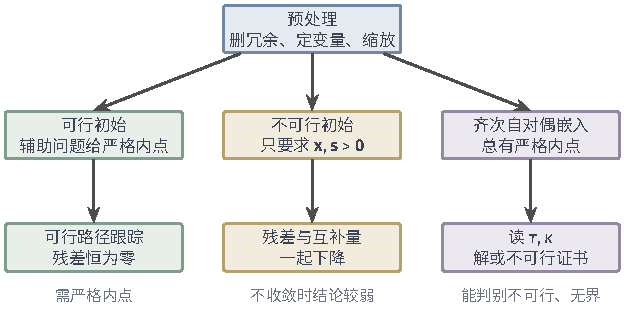
\includegraphics[width=105.738mm]{figures/05-optimization/01-linear-programming/tikz/lpipm-init-routes/figure.pdf}
  \caption{内点法起点的三条路线。预处理先去掉冗余和退化的结构。绿色路线先求严格可行点，迭代中残差恒为零；黄色路线只要求$\bm{x},\bm{s}>\bm{0}$，等式残差与互补量同时下降；紫色路线把问题嵌入一个总有严格内点的模型，由$\tau,\kappa$读出结局，并在问题不可解时给出证书。}
  \label{fig:lpipm-init-routes}
\end{BookInlineFigure}

\section{求解精度}
\label{sec:lpipm-accuracy}

内点法的迭代点永远在内部，算法只能在某一步停下来。这就需要回答：什么时候可以停，停下来的点能说明什么，以及如果需要的不是近似解而是一个基、甚至一张严格的证书，还要做什么？

\paragraph{三项残差共同决定停止}
一个点要接近最优，式~\eqref{eq:lpipm-kkt}的三组条件都要接近成立。通常用相对残差写成三条：
\begin{equation}
 \frac{\lVert\bm{A}\bm{x}-\bm{b}\rVert_2}{1+\lVert\bm{b}\rVert_2}\leq\varepsilon_{\mathrm{p}},\qquad
 \frac{\lVert\bm{A}^\top\bm{y}+\bm{s}-\bm{c}\rVert_2}{1+\lVert\bm{c}\rVert_2}\leq\varepsilon_{\mathrm{d}},\qquad
 \frac{\bm{x}^\top\bm{s}}{1+\lvert\bm{c}^\top\bm{x}\rvert}\leq\varepsilon_{\mathrm{g}}.
 \label{eq:lpipm-stop}
\end{equation}
分母里的$1$防止右端或目标恰好接近零时的除零。这些容差的意义依赖数据的尺度：把一条约束乘以$1000$，第一项的数值就改变，这和第~\ref{chap:optimization}章讨论可行性残差时指出的情况相同。

\paragraph{互补量何时是误差上界}
式~\eqref{eq:lpipm-gap-identity}的恒等式依赖两侧都可行，这时结论是干净的。

\begin{theorem}[可行点上的误差界]
\label{thm:lpipm-gap-bound}
设$\bm{x}$原始可行，$(\bm{y},\bm{s})$对偶可行。则
\begin{equation}
 0\leq\bm{c}^\top\bm{x}-p^\star\leq\bm{x}^\top\bm{s},\qquad
 0\leq d^\star-\bm{b}^\top\bm{y}\leq\bm{x}^\top\bm{s}.
 \label{eq:lpipm-gap-bound}
\end{equation}
\end{theorem}

\begin{proof}
$\bm{x}$可行给出$\bm{c}^\top\bm{x}\geq p^\star$。由弱对偶$\bm{b}^\top\bm{y}\leq d^\star\leq p^\star$，得到
\[
 \bm{c}^\top\bm{x}-p^\star\leq\bm{c}^\top\bm{x}-\bm{b}^\top\bm{y}=\bm{x}^\top\bm{s}.
\]
第二式同理，用$\bm{c}^\top\bm{x}\geq p^\star\geq d^\star$。
\end{proof}

两侧不可行时，这个界不再成立。此时
\[
 \bm{c}=\bm{A}^\top\bm{y}+\bm{s}-\bm{r}_{\mathrm{d}},\qquad\bm{b}=\bm{A}\bm{x}-\bm{r}_{\mathrm{p}}.
\]
代入目标差并整理，得到
\begin{equation}
 \bm{c}^\top\bm{x}-\bm{b}^\top\bm{y}=\bm{x}^\top\bm{s}-\bm{r}_{\mathrm{d}}^\top\bm{x}+\bm{r}_{\mathrm{p}}^\top\bm{y}.
 \label{eq:lpipm-gap-general}
\end{equation}

后两项的大小取决于残差和$\bm{x},\bm{y}$的大小。对目标误差有下面的两侧估计，它说明“残差小”换算成“目标差小”要付出什么。设$(\bm{x}^\star,\bm{y}^\star,\bm{s}^\star)$是一对最优解。

由$\bm{c}=\bm{A}^\top\bm{y}^\star+\bm{s}^\star$和$\bm{b}^\top\bm{y}^\star=p^\star$，直接计算得到
\[
 \bm{c}^\top\bm{x}-p^\star=(\bm{y}^\star)^\top\bm{r}_{\mathrm{p}}+(\bm{s}^\star)^\top\bm{x}\geq(\bm{y}^\star)^\top\bm{r}_{\mathrm{p}}.
\]
另一方面，把上面关于$\bm{c}$的表达式用到最优解$\bm{x}^\star$上，得到
\[
 p^\star=\bm{c}^\top\bm{x}^\star=\bm{b}^\top\bm{y}+\bm{s}^\top\bm{x}^\star-\bm{r}_{\mathrm{d}}^\top\bm{x}^\star.
\]
由$\bm{s}^\top\bm{x}^\star\geq0$和式~\eqref{eq:lpipm-gap-general}，得到上界。合起来就是
\begin{equation}
 (\bm{y}^\star)^\top\bm{r}_{\mathrm{p}}
 \leq\bm{c}^\top\bm{x}-p^\star
 \leq\bm{x}^\top\bm{s}+\bm{r}_{\mathrm{p}}^\top\bm{y}+\bm{r}_{\mathrm{d}}^\top(\bm{x}^\star-\bm{x}).
 \label{eq:lpipm-near-bound}
\end{equation}

这个结果的含义是，等式残差被最优解的大小放大。左端里$\bm{y}^\star$相当于影子价格：原始残差$\bm{r}_{\mathrm{p}}$相当于多用了或少用了资源，目标可以因此偏离$(\bm{y}^\star)^\top\bm{r}_{\mathrm{p}}$。所以$\bm{x}^\top\bm{s}$小并不代表目标差小，还要等式残差足够小。

图~\ref{fig:lpipm-gap-sandwich}展示了这种差别。图(a)的起点严格可行，蓝线$\bm{c}^\top\bm{x}$从上方、紫线$\bm{b}^\top\bm{y}$从下方夹住$p^\star=1$，这就是定理~\ref{thm:lpipm-gap-bound}。图(b)的起点是$\bm{x}=0.1\bm{1}$、$\bm{s}=\bm{1}$、$y=0$，等式不成立，蓝线一度在红线下方，说明此时目标值比最优值还小，并不是好事，这和第~\ref{chap:optimization}章资源分配中那个超出资源的点是同一种现象。

\begin{BookInlineFigure}
  \centering
  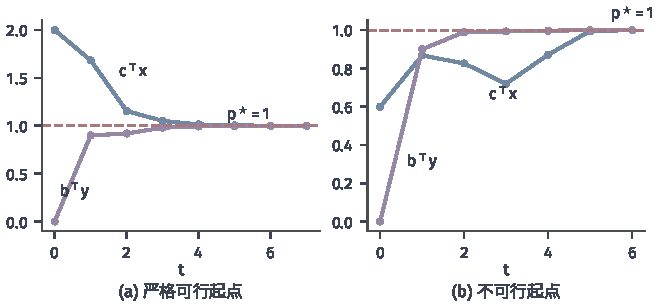
\includegraphics[width=112mm]{figures/05-optimization/01-linear-programming/matplotlib/lpipm-gap-sandwich/figure.pdf}
  \caption{原始目标（蓝）与对偶目标（紫）的夹逼，红色虚线是$p^\star=1$，$\sigma=0.3$。(a)严格可行起点，两条线从两侧夹住最优值，差距等于$\bm{x}^\top\bm{s}$。(b)不可行起点$\bm{x}=0.1\bm{1}$、$\bm{s}=\bm{1}$、$y=0$，前几轮原始目标低于最优值，原始目标甚至低于对偶目标。}
  \label{fig:lpipm-gap-sandwich}
\end{BookInlineFigure}

用图(b)的第一轮结果核对。那一点的数据是
\[
 \bm{x}\approx(0.1744,0.1521,0.1298)^\top,\qquad y=0.9,\qquad\bm{s}\approx(0.1,0.3231,0.5463)^\top,
\]
等式残差和目标值是
\[
 r_{\mathrm{p}}\approx-0.5438,\qquad\bm{r}_{\mathrm{d}}\approx(0,-0.7769,-1.5537)^\top,\qquad\bm{c}^\top\bm{x}\approx0.8678.
\]
这时$\bm{x}^\top\bm{s}\approx0.1375$是正的，但$\bm{c}^\top\bm{x}-\bm{b}^\top\bm{y}\approx-0.0322$是负的，与式~\eqref{eq:lpipm-gap-general}的右端一致。

目标误差$\bm{c}^\top\bm{x}-p^\star\approx-0.1322$落在式~\eqref{eq:lpipm-near-bound}的两端之间：左端$y^\star r_{\mathrm{p}}\approx-0.5438$，右端约为$-0.0322$。

\paragraph{近似解与精确解}
停止时得到的点满足式~\eqref{eq:lpipm-stop}，这是在给定容差和浮点运算下的结论。它和精确最优解是两回事，具体差别至少有三处。

第一，它通常不可行：$\bm{A}\bm{x}=\bm{b}$只成立到舍入误差，$\bm{x}>\bm{0}$只在严格的算术上成立。第二，它不是顶点：贯穿例第$7$轮的$x_2,x_3$是$2\times10^{-4}$和$1\times10^{-4}$，并不是零，把它们置零之后等式又不成立了。第三，浮点解的最后几位受舍入和$\bm{M}$的条件数影响，容差设得过小并不会让结果更准，反而可能使线性系统求解失败。

所以报告结果时应当把三项残差一起报告，说明容差和尺度。“求解成功”指的只是这三项达标，至于是否足够精确，要看用途。

\paragraph{基恢复}
有些用途需要一个基：要接着用单纯形法作参数分析（第~\ref{chap:simplex-method}章），要作整数规划的分支，或者需要一个顶点解。内点法不直接给出基，要从近似解转换，这一过程称为\term{基恢复}（crossover）。

做法分两阶段。先由$\hat{\bm{x}}$和$\hat{\bm{s}}$猜测哪些变量为正，例如比较$\hat{x}_i$与$\hat{s}_i$的大小，把判为零的$x_i$置零，并在其余列上修正使等式成立。然后，判为正的变量可能多于$m$个，这时沿$\bm{A}$的零空间方向移动，保持目标不变并把多余的变量逐个推到零，直到剩下的列线性无关；对偶一侧作类似的推动。最后得到一个基，用单纯形法的计算重新求出解并检查符号。

以第~\ref{sec:lpipm-central-path}节目标$\bm{c}=(0,0,1)$的例子说明。设内点法输出近似解$\hat{\bm{x}}=(0.4995,0.4995,0.001)^\top$，$\hat{\bm{s}}$的前两个分量很小，第三个分量接近$1$。比较大小后判定$x_3=0$，并修正成$(1/2,1/2,0)^\top$。

正的变量有两个，而$m=1$，还多一个。沿零空间方向$\bm{d}=(1,-1,0)^\top$移动，目标不变，走到$x_2=0$，得到顶点$(1,0,0)^\top$，基是$B=(1)$，如图~\ref{fig:lpipm-crossover}。

\begin{BookInlineFigure}
  \centering
  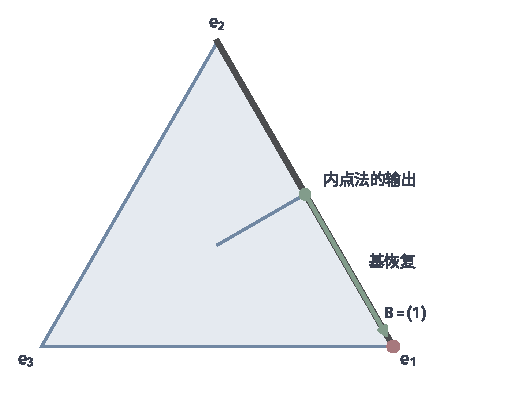
\includegraphics[width=90mm]{figures/05-optimization/01-linear-programming/matplotlib/lpipm-crossover/figure.pdf}
  \caption{基恢复的一步。目标$\bm{c}=(0,0,1)$，深灰粗线是最优边，蓝线是中心路径。内点法的输出（绿点）靠近最优边的中点，沿最优边的方向推到端点$\bm{e}_1$（红点），得到基$B=(1)$。推向$\bm{e}_2$同样得到一个最优基，所以恢复的基不唯一。}
  \label{fig:lpipm-crossover}
\end{BookInlineFigure}

用这个基作检验。$\bm{x}_B=1$，对偶是$\bm{y}=\bm{A}_B^{-\top}c_1=0$，约化成本是
\[
 \bm{s}=\bm{c}-\bm{A}^\top\bm{y}=(0,0,1)^\top\geq\bm{0},
\]
基是最优的。如果符号检验失败，从这个基继续作若干次单纯形换基。基恢复的工作量取决于$\hat{\bm{x}}$的正分量比$m$多多少，以及猜测的准确程度。已知严格互补解时恢复最优基只需多项式次运算，但实际耗时可能超过内点迭代本身。

\paragraph{精确证书}
基恢复之后得到的基和解还是浮点数算出的。如果数据是有理数，又需要严格证书，要再走一步。基矩阵$\bm{A}_B$本身是精确的，所以可以用有理数运算重新计算
\begin{equation}
 \bm{x}_B=\bm{A}_B^{-1}\bm{b},\qquad\bm{y}=\bm{A}_B^{-\top}\bm{c}_B,\qquad\bm{s}=\bm{c}-\bm{A}^\top\bm{y},
 \label{eq:lpipm-exact-check}
\end{equation}
并精确地检查$\bm{x}_B\geq\bm{0}$和$\bm{s}\geq\bm{0}$。这种检查不受任何舍入影响，通过时就是严格的最优性证明，这一点和第~\ref{chap:linear-programming}章的证书完全一致。

另一种办法是先把浮点解有理化，再验算。由Cramer法则，基本解的分母整除$\det\bm{A}_B$。两个分母都不超过$Q$的不同有理数至少相差$1/Q^2$，所以浮点解的误差只要小于$1/(2Q^2)$，分母不超过$Q$的最近有理数就只有一个，可以通过连分数求出，然后再用精确运算核对。

例如把贯穿例的约束改成$3x_1+x_2+x_3=1$，最优解是$x_1=1/3$。设内点法和基恢复给出$\hat{x}_1=0.33333341$。这里$\det\bm{A}_B=3$，分母不超过$3$的最近有理数是$1/3$。在基$B=(1)$上按式~\eqref{eq:lpipm-exact-check}作精确计算，得到
\[
 x_1=\frac13,\qquad y=\frac13,\qquad\bm{s}=\Bigl(0,\frac53,\frac83\Bigr)^\top\geq\bm{0}.
\]
这是一张可以逐项核对的最优性证书。

图~\ref{fig:lpipm-solution-pipeline}把这几个阶段连起来。算法名义上“求解完成”可以停在其中任何一个阶段，每一阶段交出的东西含义不同：近似的内部点、一个基、一个浮点最优性检验通过的基、一张严格的证书。使用结果时要分清拿到的是哪一种。

\begin{BookInlineFigure}
  \centering
  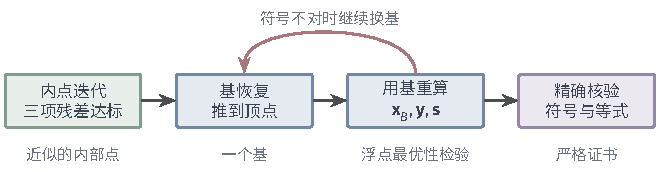
\includegraphics[width=111.739mm]{figures/05-optimization/01-linear-programming/tikz/lpipm-solution-pipeline/figure.pdf}
  \caption{从内点迭代到严格证书的各个阶段。下方灰字是每个阶段交出的结果，红色箭头表示基恢复后符号检验不通过时继续换基。}
  \label{fig:lpipm-solution-pipeline}
\end{BookInlineFigure}

\section{多项式复杂度}
\label{sec:lpipm-complexity}

单纯形法的换基次数在最坏情形下可以随维数指数增长。内点法能不能给出一个随规模温和增长的迭代次数上界？我们用最容易分析的短步路径跟踪来证明这样的界，再把它翻译成对整个算法运算量的陈述，最后指出这条界和实用规则的距离。

\paragraph{中心路径邻域}
分析的关键是不能让迭代点离路径太远，否则Newton线性化不再可靠。把“靠近路径”写成一个可以检验的条件：

\begin{definition}[中心路径的$\mathcal{N}_2$邻域]
\label{def:lpipm-neighborhood}
对$\theta\in(0,1)$，定义
\begin{equation}
 \mathcal{N}_2(\theta)=\bigl\{(\bm{x},\bm{y},\bm{s})\in\mathcal{F}^{\circ}:\lVert\bm{X}\bm{S}\bm{1}-\mu\bm{1}\rVert_2\leq\theta\mu\bigr\},
 \label{eq:lpipm-n2}
\end{equation}
其中$\mu=\bm{x}^\top\bm{s}/n$。
\end{definition}

条件说的是：把$n$个乘积看成一个向量，它偏离平均值的欧氏长度不超过平均值的$\theta$倍。中心路径上这个偏差是零。这个集合里的每个点都满足$x_is_i\geq(1-\theta)\mu>0$，所以离边界有一定的相对距离。

\paragraph{短步算法}
短步路径跟踪用可行起点，固定取单位步长，让$\mu$每轮按一个很接近$1$的比例减小：
\begin{equation}
 \sigma=1-\frac{0.4}{\sqrt{n}},\qquad\alpha=1,\qquad\theta=0.4.
 \label{eq:lpipm-short-step}
\end{equation}
这里$\sigma$必须和$\sqrt{n}$有关，直观的理由是：$\mu$的相对变化如果太大，乘积向量要移动的距离就会超出邻域。

证明的核心是控制被丢掉的二阶项$\Delta x_i\Delta s_i$。先准备一个关于向量分量乘积的引理。

\begin{lemma}[分量乘积的界]
\label{lem:lpipm-product-bound}
设$\bm{u},\bm{v}\in\mathbb{R}^n$，$\bm{u}^\top\bm{v}\geq0$。记$\bm{U}=\operatorname{diag}(\bm{u})$，$\bm{V}=\operatorname{diag}(\bm{v})$，则
\begin{equation}
 \lVert\bm{U}\bm{V}\bm{1}\rVert_2\leq2^{-3/2}\lVert\bm{u}+\bm{v}\rVert_2^2.
 \label{eq:lpipm-product-bound}
\end{equation}
\end{lemma}

\begin{proof}
把下标分成$P=\{i:u_iv_i\geq0\}$和$Q=\{i:u_iv_i<0\}$。由$\bm{u}^\top\bm{v}\geq0$，
\[
 \sum_{i\in Q}\lvert u_iv_i\rvert\leq\sum_{i\in P}u_iv_i.
\]
对$i\in P$，由$u_iv_i\leq(u_i+v_i)^2/4$，得到
\[
 \sum_{i\in P}u_iv_i\leq\frac14\sum_{i\in P}(u_i+v_i)^2\leq\frac14\lVert\bm{u}+\bm{v}\rVert_2^2.
\]
于是，用向量的$2$范数不超过$1$范数，
\[
 \lVert\bm{U}\bm{V}\bm{1}\rVert_2^2
 \leq\Bigl(\sum_{i\in P}u_iv_i\Bigr)^2+\Bigl(\sum_{i\in Q}\lvert u_iv_i\rvert\Bigr)^2
 \leq2\Bigl(\frac14\lVert\bm{u}+\bm{v}\rVert_2^2\Bigr)^2.
\]
两边开方即得。
\end{proof}

\begin{theorem}[短步路径跟踪的迭代次数]
\label{thm:lpipm-short-step}
设$(\bm{x}^{(0)},\bm{y}^{(0)},\bm{s}^{(0)})\in\mathcal{N}_2(0.4)$，按式~\eqref{eq:lpipm-newton}、\eqref{eq:lpipm-short-step}迭代。则所有迭代点都在$\mathcal{N}_2(0.4)$中，$\mu^{(t+1)}=\sigma\mu^{(t)}$，并且当
\begin{equation}
 T\geq2.5\sqrt{n}\,\log\frac{n\mu^{(0)}}{\varepsilon}
 \label{eq:lpipm-iteration-bound}
\end{equation}
时，$(\bm{x}^{(T)})^\top\bm{s}^{(T)}\leq\varepsilon$。
\end{theorem}

\begin{proof}
记当前点在$\mathcal{N}_2(\theta)$中，$\theta=0.4$，$\mu$为平均互补量。证明分四步。

\emph{第一步，二阶项的大小。}令$\bm{R}=(\bm{X}\bm{S})^{1/2}$，并定义缩放后的方向
\[
 \bm{u}=\bm{R}\bm{X}^{-1}\Delta\bm{x},\qquad\bm{v}=\bm{R}\bm{S}^{-1}\Delta\bm{s}.
\]
当前点可行，所以$\Delta\bm{x}^\top\Delta\bm{s}=0$，从而$\bm{u}^\top\bm{v}=0$。方程组第三行给出
\[
 \bm{u}+\bm{v}=\bm{R}^{-1}\bigl(\bm{S}\Delta\bm{x}+\bm{X}\Delta\bm{s}\bigr)=\bm{R}^{-1}\bigl(\sigma\mu\bm{1}-\bm{X}\bm{S}\bm{1}\bigr).
\]
由引理~\ref{lem:lpipm-product-bound}，注意到$\bm{U}\bm{V}\bm{1}=\Delta\bm{X}\Delta\bm{S}\bm{1}$，以及$\bm{R}^{-2}$的对角元不超过$1/((1-\theta)\mu)$，得到
\[
 \lVert\Delta\bm{X}\Delta\bm{S}\bm{1}\rVert_2\leq\frac{2^{-3/2}}{(1-\theta)\mu}\lVert\sigma\mu\bm{1}-\bm{X}\bm{S}\bm{1}\rVert_2^2.
\]

\emph{第二步，计算右端。}把$\sigma\mu\bm{1}-\bm{X}\bm{S}\bm{1}$写成$(\mu\bm{1}-\bm{X}\bm{S}\bm{1})-(1-\sigma)\mu\bm{1}$。两部分正交，因为$\bm{X}\bm{S}\bm{1}-\mu\bm{1}$的分量之和是$n\mu-n\mu=0$。由勾股定理和邻域条件，
\[
 \lVert\sigma\mu\bm{1}-\bm{X}\bm{S}\bm{1}\rVert_2^2\leq\theta^2\mu^2+(1-\sigma)^2n\mu^2.
\]
代入$\theta=0.4$与$(1-\sigma)^2n=0.16$，结合上一步，得到
\[
 \lVert\Delta\bm{X}\Delta\bm{S}\bm{1}\rVert_2\leq\frac{0.32}{2^{3/2}\times0.6}\,\mu<0.19\,\mu.
\]

\emph{第三步，新点仍在邻域内。}对$\alpha\in[0,1]$，记$\bm{x}(\alpha)=\bm{x}+\alpha\Delta\bm{x}$，$\bm{s}(\alpha)$同理。由第三行，
\[
 x_i(\alpha)s_i(\alpha)=(1-\alpha)x_is_i+\alpha\sigma\mu+\alpha^2\Delta x_i\Delta s_i.
\]
前两项之和不小于$\min\{(1-\theta)\mu,\sigma\mu\}\geq0.6\mu$（$n\geq1$时$\sigma\geq0.6$），第三项的绝对值不超过$0.19\mu$，所以$x_i(\alpha)s_i(\alpha)>0$。乘积从正数出发一直为正，$x_i(\alpha)$和$s_i(\alpha)$就不能变号，因此$\bm{x}^+,\bm{s}^+>\bm{0}$。

$\Delta\bm{x}^\top\Delta\bm{s}=0$说明$\mu^+=\sigma\mu$。$\alpha=1$时，上面的展开给出$x_i^+s_i^+-\sigma\mu=\Delta x_i\Delta s_i$，于是
\[
 \lVert\bm{X}^+\bm{S}^+\bm{1}-\mu^+\bm{1}\rVert_2<0.19\,\mu\leq0.4\,\sigma\mu=\theta\mu^+,
\]
最后一步用到$0.4\sigma\geq0.24$。等式约束由线性性保持，所以新点在$\mathcal{N}_2(0.4)$中。

\emph{第四步，计数。}由上面的结论，$n\mu^{(T)}=n\sigma^T\mu^{(0)}$。利用$\log(1-\beta)\leq-\beta$，只要式~\eqref{eq:lpipm-iteration-bound}成立，就有
\[
 n\mu^{(T)}\leq n\mu^{(0)}\exp\Bigl(-\frac{0.4\,T}{\sqrt{n}}\Bigr)\leq\varepsilon.\qedhere
\]
\end{proof}

这个定理的结构可以这样概括：$\theta$保证Newton步的二阶项足够小，$\sigma$的取法让一步能被邻域容纳，两者的相容性来自$\sqrt{n}$这个因子。由于$(1-\sigma)^2n$要固定，每步减少的比例只能是$1/\sqrt{n}$量级，这就是迭代次数含$\sqrt{n}$的原因。

以贯穿例验证。从中心点$\bm{x}^{(0)}=(6/11,3/11,2/11)^\top$、$y^{(0)}=0$出发，$n=3$，$\sigma=1-0.4/\sqrt{3}\approx0.7691$，起点和前两轮的$\mu$是$0.5455$、$0.4195$、$0.3226$，每轮都乘以$\sigma$。全程相对偏差的最大值约为$0.045$，远小于$0.4$。

取$\varepsilon=10^{-3}$，式~\eqref{eq:lpipm-iteration-bound}给出的上界是
\[
 2.5\sqrt{3}\,\log\frac{18/11}{10^{-3}}\approx32.04,
\]
实际用了$29$轮。短步规则的实际轮数几乎就是理论值，因为$\sigma$是预先固定的。作为对照，第~\ref{sec:lpipm-path-following}节同一个问题用预测—校正把互补量降到$10^{-3}$以下只需$4$轮。

\paragraph{从迭代次数到运算量}
式~\eqref{eq:lpipm-iteration-bound}只计迭代次数。要说“线性规划可以在多项式时间内求解”，还要计入每一轮的代价和数字的长度。整个结论由下面三部分拼成。

第一是每轮的算术运算量：解一个$m\times m$的稠密方程组，需要$O(n^3)$次算术运算（$m\leq n$）。第二是迭代次数中的$\log(n\mu^{(0)}/\varepsilon)$，要说清起点和精度是多少。

第三部分是输入的位长。设数据全部是整数，写出整个问题需要$L$个二进制位，这里$L$至少是$m,n$和各系数位数的总和。可以证明两件事：存在满足定理条件的起点，其$\mu^{(0)}$不超过$2^{O(L)}$，这类起点由第~\ref{sec:lpipm-initial-point}节的嵌入构造给出；只要把间隙降到$2^{-O(L)}$以下，由于有理顶点的分母有界，就可以把近似解精确地修整成最优基。

把这三部分合起来，得到迭代次数$O(\sqrt{n}L)$，算术运算总量$O(n^{3.5}L)$，运算中只需保留$O(L)$位的精度，总的二进制运算量是$L$和$n$的多项式。严格的推导要逐项跟踪精度和起点，篇幅较长，读者可查阅专著\scite{math-bertsimas1997linear}。

这里“多项式”的含义要说准。上面的界依赖$L$，也就是系数的位数，所以这是位模型下的多项式时间，又称弱多项式。是否存在迭代次数只依赖$m,n$、不依赖系数位长的线性规划算法，至今仍是公开问题。内点法的$\log(1/\varepsilon)$项在这里起作用：想要精确解，就需要把精度推到由$L$决定的程度。

\paragraph{理论规则与实用规则}
短步规则的上界最好，实际却很慢：它每轮只减小约$0.4/\sqrt{n}$，从不利用可以走更远的情况。放宽邻域能让步子变大。定义单侧邻域
\begin{equation}
 \mathcal{N}_{-\infty}(\gamma)=\bigl\{(\bm{x},\bm{y},\bm{s})\in\mathcal{F}^{\circ}:x_is_i\geq\gamma\mu,\ i=1,\ldots,n\bigr\},\quad\gamma\in(0,1).
 \label{eq:lpipm-n-inf}
\end{equation}
$\gamma$很小时，几乎只要求每个乘积不要低于平均值太多。图~\ref{fig:lpipm-neighborhoods}(a)是$n=2$时两种邻域在乘积平面上的形状：$\mathcal{N}_2$是窄条，$\mathcal{N}_{-\infty}$几乎占满整个象限。

\begin{BookInlineFigure}
  \centering
  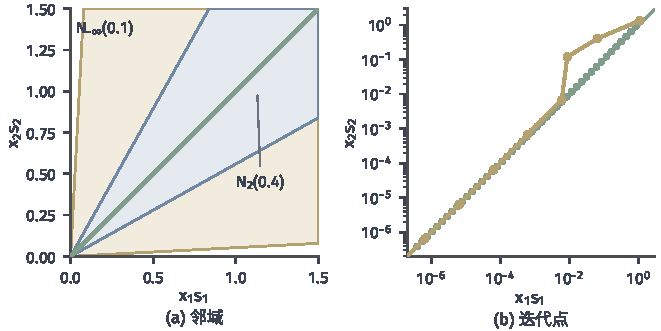
\includegraphics[width=112mm]{figures/05-optimization/01-linear-programming/matplotlib/lpipm-neighborhoods/figure.pdf}
  \caption{$n=2$时中心路径的邻域，横纵轴是两个乘积$x_1s_1,x_2s_2$，绿色对角线是中心路径。(a)蓝色是$\mathcal{N}_2(0.4)$，黄色是$\mathcal{N}_{-\infty}(0.1)$。(b)问题$\min x_1+2x_2$、$x_1+x_2=1$上的迭代点，对数坐标。绿点是短步规则，黄点是$\sigma=0.1$的长步规则，长步规则离路径更远，点数少得多。}
  \label{fig:lpipm-neighborhoods}
\end{BookInlineFigure}

在$\mathcal{N}_{-\infty}(\gamma)$上，每轮取较小的$\sigma$，再沿方向走到将要离开邻域为止，称为长步路径跟踪。它的理论上界是$O(n\log(1/\varepsilon))$，比短步的$O(\sqrt{n}\log(1/\varepsilon))$差，实际表现却远好于短步。

第~\ref{sec:lpipm-path-following}节的预测—校正规则则按式~\eqref{eq:lpipm-sigma-rule}自适应地选$\sigma$，加上二阶校正。按通常的写法，它没有多项式的迭代次数保证，但它是大规模求解器的常用方案。

图~\ref{fig:lpipm-iteration-growth}是随机线性规划上的迭代次数。每个问题都从同一个中心点出发，要求$\mu\leq10^{-6}$。短步规则的轮数紧贴理论值，随$\sqrt{n}$增长，$n=1000$时超过一千轮。长步规则和预测—校正增长得慢得多，$n=1000$时只需$23$轮和$12$轮。

\begin{BookInlineFigure}
  \centering
  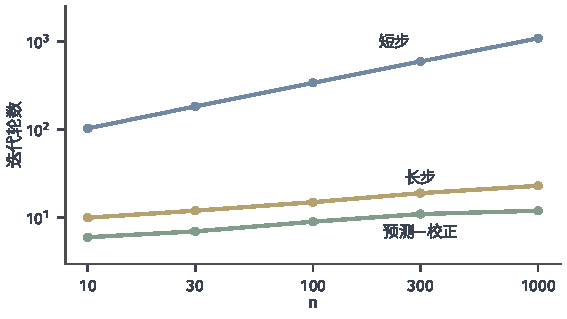
\includegraphics[width=96mm]{figures/05-optimization/01-linear-programming/matplotlib/lpipm-iteration-growth/figure.pdf}
  \caption{随机稠密线性规划上三种规则的迭代轮数，$m=n/2$，对数坐标，起点$\bm{x}=\bm{s}=\bm{1}$是中心点，停止条件$\mu\leq10^{-6}$。蓝线是短步规则，黄线是长步规则（$\sigma=0.1$、$\gamma=10^{-3}$），绿线是预测—校正。每个$n$只运行一个固定种子的实例，用来展示量级而不是平均表现。}
  \label{fig:lpipm-iteration-growth}
\end{BookInlineFigure}

表~\ref{tab:lpipm-rules}把三者放在一起。理论界最好的规则不是实践中最快的规则，这个差距是内点法的一个基本事实。

\begin{BookInlineTable}
  \centering
  \begin{tabular}{@{}llll@{}}
    \toprule
    规则 & 邻域 & 迭代上界 & 实践表现\\
    \midrule
    短步 & $\mathcal{N}_2(0.4)$ & $O(\sqrt{n}\log(1/\varepsilon))$ & 接近理论值，很慢\\
    长步 & $\mathcal{N}_{-\infty}(\gamma)$ & $O(n\log(1/\varepsilon))$ & 轮数少\\
    预测—校正 & 无固定邻域 & 无一般保证 & 通常最少\\
    \bottomrule
  \end{tabular}
  \caption{三种路径跟踪规则的比较。上界针对可行起点；预测—校正指式~\eqref{eq:lpipm-sigma-rule}的常用写法，加上保护措施的变体可以恢复多项式界。}
  \label{tab:lpipm-rules}
\end{BookInlineTable}

\paragraph{历史上的位置}
线性规划的多项式可解性最早不是由内点法确立的。1979年，Khachiyan用椭球法证明了线性规划可以在多项式时间内求解，这个方法每步用一个椭球包住可能的解集，并不断缩小椭球。它在理论上解决了问题，实际计算却很慢。

1984年Karmarkar提出的算法同样具有多项式复杂度，并且在实践中有竞争力，随后的工作发展出本章的原始—对偶路径跟踪。这段历史可以帮助分清两件事：多项式界回答“最坏情形下随规模怎样增长”，实际快慢还取决于常数、结构和实现。

\section{单纯形法与内点法的比较}
\label{sec:lpipm-comparison}

现在两种算法都有了。于是要问：面对一个具体的线性规划，两者各需要做什么、各能交出什么？我们先在同一个工厂问题上把它们并排算一遍，再按稀疏性、内存、退化和再求解几个方面对比。

\paragraph{同一个问题上的两种计算}
工厂问题的标准型是第~\ref{chap:simplex-method}章的数据，$m=3$，$n=5$，最优解是$(4,2,0,0,1)^\top$，最优利润$26$，对偶最优解$\bm{y}^\star=(-2,-1,0)^\top$。单纯形法从基$(3,4,5)$出发，经过$(0,3)$、$(2,3)$，$3$次换基到达最优顶点，每次换基求解一个$3\times3$的基矩阵方程组。

内点法取严格可行起点
\[
 \bm{x}^{(0)}=(1,1,5,7,2)^\top,\qquad\bm{y}^{(0)}=(-3,-3,-3)^\top,\qquad\bm{s}^{(0)}=(5,7,3,3,3)^\top,
\]
这里$\bm{s}^{(0)}=\bm{c}-\bm{A}^\top\bm{y}^{(0)}$，$\mu^{(0)}=10.8$。第一轮的正规矩阵是
\[
 \bm{M}=\bm{A}\bm{D}\bm{A}^\top\approx
 \begin{bmatrix}2.4381&0.6857&0.2857\\0.6857&3.2762&0.1429\\0.2857&0.1429&0.8095\end{bmatrix}.
\]

两种算法都在解$3\times3$的对称或非对称方程组，表面上规模一样，含义却不同。基矩阵只用$\bm{A}$的$3$列，换基时只变一列；$\bm{M}$用到全部$5$列，每轮的数值都变，但元素的稀疏结构不变。

用预测—校正（$\eta=0.99$），$6$轮后互补量从$54$降到约$1.2\times10^{-7}$，点在$4$位小数上就是$(4,2,0,0,1)^\top$。

图~\ref{fig:lpipm-factory-run}把这两个过程画在一起。单纯形法的每一步都站在顶点上，利润单调上升，$3$步后得到精确解。内点法的头几轮就穿过内部接近最优点，第$3$轮已到$25.95$，但此后每轮只是把小数位往后推，点始终不是顶点。

\begin{BookInlineFigure}
  \centering
  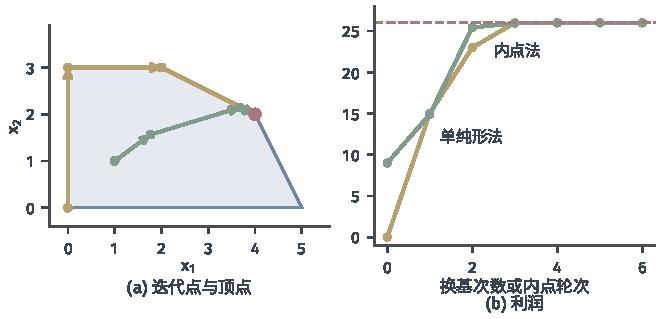
\includegraphics[width=112mm]{figures/05-optimization/01-linear-programming/matplotlib/lpipm-factory-run/figure.pdf}
  \caption{工厂问题上的两种算法。(a)可行域上，黄色是单纯形法的顶点序列，绿色是内点法的前几个迭代点，红点是最优顶点$(4,2)$。(b)利润随迭代的变化，黄线是单纯形法的换基次数，绿线是内点法的轮次，红色虚线是最优值$26$。单纯形法的横轴单位是一次换基，内点法的单位是一次分解$\bm{M}$，两者的代价不同，不能只比轮次。}
  \label{fig:lpipm-factory-run}
\end{BookInlineFigure}

\paragraph{稀疏存储与分解填充}
大规模线性规划的矩阵$\bm{A}$几乎都是稀疏的，这时代价取决于分解时产生多少新的非零元（填充）。两种算法的填充模式不同。

单纯形法分解基矩阵，用LU分解并在换基时更新，只涉及$m$列。内点法分解$\bm{A}\bm{D}\bm{A}^\top$，它的第$(i,k)$个元素非零，当且仅当存在一列在第$i$行和第$k$行都非零。于是只要$\bm{A}$有一列稠密，$\bm{M}$就整个稠密。

图~\ref{fig:lpipm-sparsity}是一个例子：$\bm{A}$是$40\times80$的稀疏矩阵，每列只有两个非零元，再加上一个稠密列。整个$\bm{A}$只有$198$个非零元，$\bm{M}$却有全部$1600$个；去掉那一列后，$\bm{M}$只有$196$个非零元。实现中会把稠密列单独分离出来，用矩阵求逆引理处理，但这需要额外的数值稳定措施。

\begin{BookInlineFigure}
  \centering
  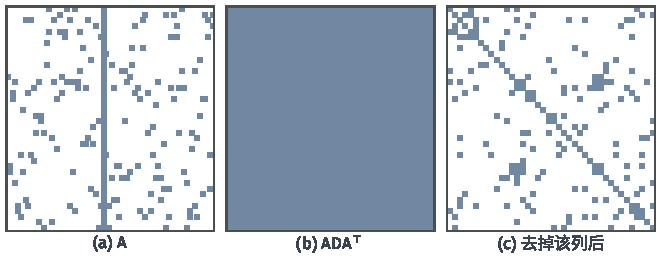
\includegraphics[width=112mm]{figures/05-optimization/01-linear-programming/matplotlib/lpipm-sparsity/figure.pdf}
  \caption{一个稠密列的影响，蓝色方块表示非零元。(a)$40\times80$的稀疏矩阵$\bm{A}$，其中一列稠密。(b)正规矩阵$\bm{A}\bm{D}\bm{A}^\top$完全稠密。(c)去掉该列后的$\bm{A}\bm{D}\bm{A}^\top$仍然稀疏。}
  \label{fig:lpipm-sparsity}
\end{BookInlineFigure}

\paragraph{内存}
内点法每轮要存$\bm{M}$的Cholesky因子，内存由填充决定，并且在整个求解期间都要占用这么多。单纯形法只存基的LU因子，通常比前者小，但可能需要很多次换基。所以问题规模增大时，内点法更容易受内存限制，单纯形法更容易受迭代次数限制，具体哪个先成为瓶颈取决于矩阵结构。

\paragraph{退化与数值性质}
第~\ref{chap:simplex-method}章说明，退化时单纯形法可能原地换基，需要反循环规则。内点法从不访问顶点，路径本身不受退化的基影响，第$t$轮的$\bm{D}$只和当前点有关，因此没有“卡在同一顶点”的现象。

内点法的麻烦在别处。$\bm{D}$的对角元是$x_i/s_i$，随迭代趋于两个极端：最优解中为正的变量对应的元素趋于$+\infty$，为零的变量对应的元素趋于$0$。图~\ref{fig:lpipm-scaling-spread}(a)显示，工厂问题最后几轮对角元的比值已超过$10^{20}$。

\begin{BookInlineFigure}
  \centering
  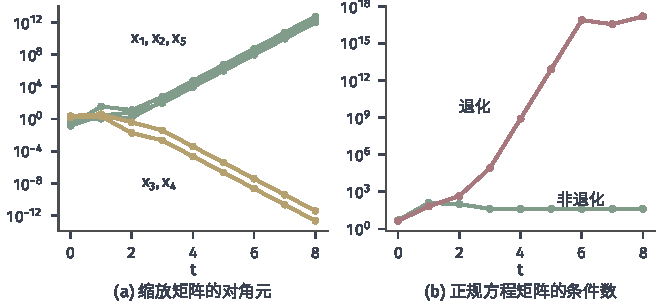
\includegraphics[width=112mm]{figures/05-optimization/01-linear-programming/matplotlib/lpipm-scaling-spread/figure.pdf}
  \caption{缩放矩阵与条件数的变化，预测—校正，$\eta=0.99$。(a)工厂问题中$D_{ii}=x_i/s_i$随轮次的变化，绿线对应最优解中为正的$x_1,x_2,x_5$，黄线对应为零的$x_3,x_4$。(b)$\bm{M}=\bm{A}\bm{D}\bm{A}^\top$的$2$范数条件数：绿线是非退化的工厂问题，红线是再加一条约束$x_1+x_2\leq6$使最优顶点退化的情形。}
  \label{fig:lpipm-scaling-spread}
\end{BookInlineFigure}

这种悬殊看起来很危险，影响却取决于问题的结构。图~\ref{fig:lpipm-scaling-spread}(b)的绿线说明，非退化时$\bm{M}$由三个正的基变量主导，它们的$D_{ii}$同步增大，条件数稳定在约$41$。红线是最优顶点退化的情形，正变量少于$m$个，$\bm{M}$趋于奇异，条件数涨到$10^{16}$以上。

大的条件数并不直接意味着算出的方向没用：误差往往落在对后续更新影响不大的子空间里，这是内点法在实践中比条件数预示的更稳健的原因，但这需要专门的误差分析，读者可查阅专著\scite{math-nocedal2006numerical}。求解器还要辅以正则化和迭代精化。最终都应当检查残差，不能只凭条件数判断。

\paragraph{基与再求解}
单纯形法返回一个基，这使很多后续工作很方便：约束或目标有微小改变时，从原来的基接着做，往往几次换基就够（第~\ref{chap:simplex-method}章的对偶单纯形法）；固定基的参数分析可以直接读出结论成立的范围。

内点法也返回对偶信息，这些$\bm{y}$和$\bm{s}$的值可以当作影子价格用，但结果是最优面中央的一个点，解不唯一时它和某个基给出的对偶解并不相同。需要基时要做上一节的基恢复。

内点法的热启动也比较困难。上一次的解贴近边界，某些$x_i$或$s_i$接近零，从这里出发的步长通常很短，反而不如重新开始。因此在分支限界这类需要大量相关求解的场景中，单纯形法更占优势，这也是两种方法长期并存的原因之一。

\paragraph{速度取决于问题和实现}
两种算法都不总是更快。一般而言，内点法在规模很大且$\bm{M}$稀疏时往往轮数少、速度快，单纯形法在$\bm{M}$稠密或需要反复热启动时更有优势。这只是经验性的倾向，具体结果要看矩阵结构、预处理和实现水平，求解器通常提供两者甚至并行运行。

表~\ref{tab:lpipm-compare}总结了本节的对比。

\begin{table*}[!htbp]
  \centering
  \begin{tabular}{@{}lll@{}}
    \toprule
    方面 & 单纯形法 & 内点法\\
    \midrule
    每步的工作 & 解基矩阵方程，换一列 & 分解$\bm{A}\bm{D}\bm{A}^\top$，全部列参与\\
    迭代次数 & 随结构变化，最坏情形指数 & 通常很少，短步规则有$O(\sqrt{n}\log(1/\varepsilon))$的界\\
    稀疏结构 & 基的LU因子，变化较小 & 稠密列会使$\bm{M}$稠密，需特殊处理\\
    内存 & 通常较小 & 由Cholesky填充决定，通常较大\\
    退化 & 可能原地换基，需反循环规则 & 不停滞，但$\bm{M}$可能病态\\
    交出的结果 & 基、顶点解、对偶解 & 内部的近似点和对偶量，需要基时另作恢复\\
    再求解 & 从旧基热启动较容易 & 从旧解热启动较困难\\
    \bottomrule
  \end{tabular}
  \caption{单纯形法与内点法的对比。各项是对典型情形的概括，速度结论取决于问题结构和实现。无论用哪种方法，浮点实现都要检验可行性和最优性。}
  \label{tab:lpipm-compare}
\end{table*}

\section{本章小结}
\label{sec:lpipm-summary}

本章开头问：能不能不贴着边走，从可行域的内部穿过去？答案是把互补松弛$x_is_i=0$放宽成$x_is_i=\mu$。原始和对偶都有严格可行点时，这组方程对每个$\mu>0$有唯一解，解连成中心路径，沿路径的对偶间隙恰好是$n\mu$。路径的极限是一对严格互补的最优解，落在最优面的解析中心，解不唯一时并不是顶点。

沿路径前进靠Newton法。线性化$x_is_i=\sigma\mu$得到一个由原始残差、对偶残差和互补残差驱动的线性方程组，消元后只需解$m\times m$的对称正定方程$\bm{A}\bm{D}\bm{A}^\top\Delta\bm{y}=\bm{h}$。到边界的比例规则保持$\bm{x},\bm{s}>\bm{0}$，$\sigma$在减小互补量和靠近中心之间折中，预测—校正用一次试算选定$\sigma$并补偿二阶项，两次求解共用一次分解。

这些步骤合起来是一个完整的求解过程。起点可以严格可行，也可以只要求正性，让等式残差和互补量一起下降；需要判别不可行或无界时，用预处理和齐次自对偶嵌入。停止时要同时看三项残差，只有在原始、对偶都可行时，$\bm{x}^\top\bm{s}$才是目标误差的上界，否则还要计入等式残差被最优解放大的部分。

交付的结果有几个层次，它们的含义不同：浮点容差下的近似解，基恢复之后的基，用精确算术核对过的证书。理论方面，短步路径跟踪的迭代次数不超过$O(\sqrt{n}\log(n\mu^{(0)}/\varepsilon))$，配合起点构造和位长分析得到线性规划的多项式算法；椭球法更早建立了这一可解性。理论规则和实用的预测—校正之间有明显差距，不能把后者的经验速度当作定理。

选择算法时，单纯形法便于热启动、返回基，适合反复求解和灵敏度分析；内点法迭代次数少，适合大规模稀疏问题，但对$\bm{A}\bm{D}\bm{A}^\top$的填充敏感，需要基时要另作恢复。两者都需要在最后检验可行性和最优性。

路径跟踪的思路并不限于线性规划。当约束是一般的光滑函数或锥时，障碍和扰动互补仍然可用，但方程不再是双线性的，Newton系统含有Hessian和Jacobian的变化，严格内点、初值和停止证书都有新的条件，这些由第~\ref{chap:nonlinear-interior-point}章展开。

